\subsection{Pre-selection and event cleaning}
\label{subsec:sec.strategy.selection_cleaning}

A sample of two same-sign or three leptons is selected applying the following criteria:
\begin{itemize}
\item[$\bullet$] \textbf{Jet Cleaning}: 
Events are required to pass a set of cleaning requirements. 
An event is rejected if any pre-selected jets ($|\eta|<4.9$, after 
jet-electron overlap removal) fails the jet quality criteria. 
The cleaning requirements are intended to remove events where significant 
energy was deposited in the calorimeters 
due to instrumental effects such as cosmic rays, beam-induced (non-collision) 
particles, and noise. Around 0.5\% of data events are lost after applying 
this cut.

\item \textbf{Primary Vertex}:
Events are required to have a reconstructed vertex~\cite{ATL-PHYS-PUB-2015-026} 
with at least two associated tracks with $\pt >400$~MeV. The vertex with the largest $\Sigma \pt^2$ of the associated tracks 
is chosen as the primary vertex of the event.
This cut is found to be 100\% efficient.

\item \textbf{Bad Muon Veto}: 
Events containing at least one pre-selected muon satisfying $\sigma(q/p)/|q/p| >$ 0.2 before the overlap removal are rejected. 
Around 0.1\% of data events are removed by this cut.

\item \textbf{Cosmic Muon Veto}: 
Events containing a cosmic muon candidate are rejected. 
Cosmic muon candidates are looked for among pre-selected muons, 
if they fail the requirements $|z_0| <1.0$ mm and $|d_0|<0.2$ mm, 
where the longitudinal and transverse impact parameters $z_0$ and $d_0$ 
are calculated with respect to the primary vertex. 
Up to 6\% of data events are lost at this cleaning cut.

\item \textbf{At least two leptons}: 
Events are required to contain at least two signal leptons 
with $\pt>20 \GeV$ for the two leading leptons. 
If the event contains a third signal lepton with $\pt>10 \GeV$ the event is regarded as a three-lepton event, otherwise as a two-lepton event. 
The data sample obtained is then divided into three channels depending on the flavor of the two  leptons forming a same-sign pair ($ee$, $\mu\mu$, $e\mu$). 
If more than one same-sign pairs can be built, the one involving the leading 
lepton will be considered for the channel selection. 

\item \textbf{Same-sign}: 
if the event has exactly two leptons, then these two leptons
 have to be of identical electric charge (``same-sign'').
\end{itemize}

The following event variables are also used in the definition of the signal and validation regions in the analysis:
\begin{itemize}
\item The inclusive effective mass \meff~ defined as the scalar sum of
  all the signal leptons \pt , all signal jets \pt\ and \met. 
\end{itemize}

\subsection{Trigger strategy}
\label{subsec:sec.strategy.sel.selection_trigger}
  
Events are selected using a combination of dilepton and $\met$ triggers, the latter being used only for events with $\met>250 \GeV$. 
Since the trigger thresholds have been raised between 2015 and 2016 due to the 
continuous increase of the instantaneous luminosity, 
the dilepton triggers used for: 
\begin{itemize}
\item 2015 data:
logical \texttt{or} of a trigger with two electrons of 12 \GeV, 
with an electron of 17 \GeV~and a muon of 14 \GeV,
with two muons of 18 \GeV~and 8 \GeV. 
\item 2016 data:
logical \texttt{or} of a trigger with two electrons of 17 \GeV, 
with an electron of 17 \GeV~and a muon of 14 \GeV,
with two muons of 22 \GeV~and 8 \GeV. 
\end{itemize}
The $\met$ trigger was also raised from 70\GeV~to a 100 \GeV~and 110 \GeV.
The trigger-level requirements on $\met$ and the leading and subleading lepton \pt are looser than those applied offline 
to ensure that trigger efficiencies are constant in the relevant phase space.

%In MC, the configuration is chosen randomly between the different options, 
%according to the relative luminosities and $\langle\mu\rangle$ profiles of 
%the 2015 and 2016 datasets. 

\par{\bfseries Trigger matching\\}
For events exclusively selected via one or several of the dilepton triggers, 
we require a matching between the online and offline leptons with $\pt>20 \GeV$.
with the exception of the di-muon trigger for which muons with $\pt>10 \GeV$ 
are also considered.
In addition, for the di-muon trigger in the 2016 configuration, 
the \pt\ requirement of the leading matched muon is raised to 23 \GeV~
to remain on the trigger efficiency plateau. 

\par{\bfseries Trigger scale factors\\}
The simulated events are corrected for any potential differences in 
the trigger efficiency between data and MC simulation.
Assuming no correlation between the \met\ and dilepton triggers, 
trigger scale factors are applied to MC events which were not selected 
by the \met\ trigger.
These scale factors are computed for each event, considering the combination of fired triggers, the number and flavours of the leptons, 

\subsection{Object definition}
\label{subsec:strategy.sel.obj}

This section presents the definitions of the objects used in the analysis: 
jets, electrons, muons and $\met$ (the taus are not considered).

\subsection*{Jets}
\label{subsec:sec.strategy.sel.objects_jets}



The jets are kept only if they have $p_\mathrm{T}>20$~GeV~and lie 
within $|\eta|<2.8$. 
To mitigate the effects of pileup, the pile-up contribution is subtracted 
from the expected average energy contribution according to the jet area~\cite{Cacciari:2007fd,Aaboud:2017jcu}.
In order to reduce the effects of pile-up, 
a significant fraction of the tracks in jets with $\pt<60 \GeV$ and $|\eta|<2.4$ must originate from the primary vertex, 
as defined by the jet vertex tagger (JVT)~\cite{ATLAS-CONF-2014-018}. 
The jet calibration follows the prescription in Ref.~\cite{Aaboud:2017jcu}.

 
The 70\% efficiency operating point of the MV2c10 algorithm  was chosen which 
corresponds to the
average efficiency for tagging $b$-jets in simulated $\ttbar$ events. 
This efficiency working point was favored by optimisation studies performed in 
simulated signal and background samples.
The rejection factors for light-quark/gluon jets, $c$-quark jets and hadronically decaying $\tau$ leptons in simulated $\ttbar$ events 
are approximately 380, 12 and 54, respectively~\cite{ATL-PHYS-PUB-2015-022,ATL-PHYS-PUB-2016-012}. 
Jets with $|\eta|<2.5$ which satisfy the $b$-tagging and JVT requirements are identified as $b$-jets. 
Correction factors and uncertainties determined from data for the $b$-tagging efficiencies and mis-tag rates
are applied to the simulated samples~\cite{ATL-PHYS-PUB-2015-022}. 

For the data-driven background estimations, two categories of electrons and muons are used: 
``candidate'' and ``signal'' with the latter being a subset of the ``candidate'' leptons satisfying tighter selection criteria. 

\subsection*{Electrons}
\label{subsec:sec.strategy.sel.objects_electrons}

Electron candidates are reconstructed from energy depositions in the 
electromagnetic calorimeter and required to be matched to an 
inner detector track, 
to have $\pT> 10 \GeV$ and $|\eta|<2.47$, and to pass the 
``Loose'' likelihood-based electron identification 
requirement~\cite{ATLAS-CONF-2016-024}.
Electrons in the transition region between the barrel and endcap 
electromagnetic calorimeters ($1.37<|\eta|<1.52$) are rejected to reduce 
the contribution from fake/non-prompt electrons. 
The transverse impact parameter $d_0$ 
with respect to the reconstructed primary vertex 
must satisfy $|d_0/\sigma(d_0)|<5$.
This last requirement helps reduce the contribution from charge 
mis-identification. 

Signal electrons are additionally required to pass the ``Medium'' 
likelihood-based identification requirement~\cite{ATLAS-CONF-2016-024}.
Only signal electrons with $|\eta|<2.0$ are considered, 
to reduce the level of charge-flip background.
In addition, signal electrons that are likely to be reconstructed with an incorrect charge assignment are rejected using a few electron cluster and track properties: the track impact parameter, the track curvature significance, the cluster width and the quality of the matching between the cluster and its associated track, both in terms of energy and position. These variables, as well as the electron \pt and $\eta$, are combined into a single classifier using a boosted decision tree (BDT). A selection requirement on the BDT output is chosen such as to achieve a rejection factor between 7 and 8 for electrons with a wrong charge assignment while selecting properly measured electrons with an efficiency of 97\% (in $Z\rightarrow ee$ MC). 

A multiplicative event weight is applied for each signal electron in MC to the overall event weight 
in order to correct for differences in efficiency between data and MC.

\subsection*{Muons}
\label{subsec:sec.strategy.sel.objects_muons}

Muons candidates are reconstructed from muon spectrometer tracks matched to 
the inner detector tracks in the region $|\eta|<2.5$.
Muon candidates must pass the ``Medium'' identification 
requirements~\cite{Aad:2016jkr} and have  $p_\mathrm{T} > 10\GeV$ and 
$|\eta| < 2.4$. 
Signal muons are required to pass $\vert d_0\vert/\sigma(d_0) < 3$
and $|z_0 \cdot\sin(\theta)|<0.5 mm$.
 
A multiplicative event weight is applied for each selected muon in MC to the overall event weight 
in order to correct for differences in efficiency between data and MC.

\subsection*{Overlap removal}
\label{subsec:sec.strategy.sel.objects_overlap_removal}

According to the above definitions, one single final state object may fall in more than one category, being therefore effectively double-counted. 
For example, one isolated electron is typically reconstructed both as an electron and as a jet. 
A procedure to remove overlaps between final state objects was therefore put in place, and applied on pre-selected objects. 
Any jet within a distance $\Delta R_y \equiv \sqrt{(\Delta y)^2+(\Delta\phi)^2} =$ 0.2 of a lepton candidate is discarded, 
unless the jet is $b$-tagged,\footnote{In this case the $b$-tagging operating point corresponding to an efficiency of 85\% is used.} 
in which case the lepton is discarded since it probably originated from a semileptonic $b$-hadron decay. 
Any remaining lepton within $\Delta R_y \equiv \operatorname{min}\{0.4, 0.1 + 9.6 \GeV/\pt(\ell)\}$ of a jet is discarded. 
In the case of muons, the muon is retained and the jet is discarded if the jet has fewer than three associated tracks. This reduces 
inefficiencies for high-energy muons undergoing significant energy loss in the calorimeter. 

\subsection*{Missing transverse energy}
\label{subsec:sec.strategy.sel.objects_met}

The missing transverse energy (\met) is computed as a negative vector sum of 
the transverse momenta 
of all identified candidate objects (electrons, photons~\cite{Aaboud:2016yuq}, muons and jets) and an additional soft term. 
The soft term is constructed from all tracks associated with the primary vertex but not with any physics object. 
In this way, the $\met$ is adjusted for the best calibration of the jets and the other identified physics objects listed above, 
while maintaining approximate pile-up independence in the soft term~\cite{ATL-PHYS-PUB-2015-027, ATL-PHYS-PUB-2015-023}.

\subsection{Data-MC comparisons}
\label{subsec:sec.strategy.selection_DataMC}


In order to validate the various choices made regarding the object definitions and event selection, 
check their sensible behavior and their reasonable modelling in the simulations, 
we looked at the distributions of several kinematic variables obtained with the full available data set.
Figures~\ref{fig:dataMC_2lep}-\ref{fig:dataMC_metmeff} show such selected distributions in data compared to MC. 
The background distributions are taken directly from MC with no data-driven estimation of the charge flip or non-prompt lepton backgrounds.

Figure~\ref{fig:dataMC_2lep} shows the dilepton invariant mass distributions for both opposite-sign (OS) and same-sign (SS) dilepton events, 
computed with the two leading $p_T$ leptons. 
A very good agreement with MC is observed in the OS channels, with a clear $Z$-boson mass peak in the $ee$ and $\mu\mu$ channels. 
In the SS channels, the $Z$-boson mass peak is also observed in the $ee$ channel due to electron charge mis-identification, with MC overestimating data. 
% by 20-30\%. 
An accumulation of events at the $Z$-boson mass is also observed in the SS $e\mu$ and $\mu\mu$ channels due to three-lepton events 
from either $Z$+jets with a fake lepton or from $WZ$ production.  

The transverse momentum distributions of the signal leptons used in the analysis are shown in Figure~\ref{fig:dataMC_lep1}, with a reasonable data-MC agreement except at low 
lepton $\pt$ where some discrepancies and accumulation of events involving fake leptons ($Z$+jets, $W$+jets, $\ttbar$) are observed. 
%Jet and $b$-jet distributions are shown in Figures~\ref{fig:dataMC_jet}-\ref{fig:dataMC_bjet} 
Figure~\ref{fig:dataMC_metmeff} shows the $\met$ and $m_{\rm eff}$ distributions.

The background estimation, in Chapter ~\ref{chap:fake} and Chapter~\ref{chap:bkg}, will be dedicated to improving the estimates of the background prediction using data-driven methods.

\begin{figure}[htb!]
\centering
{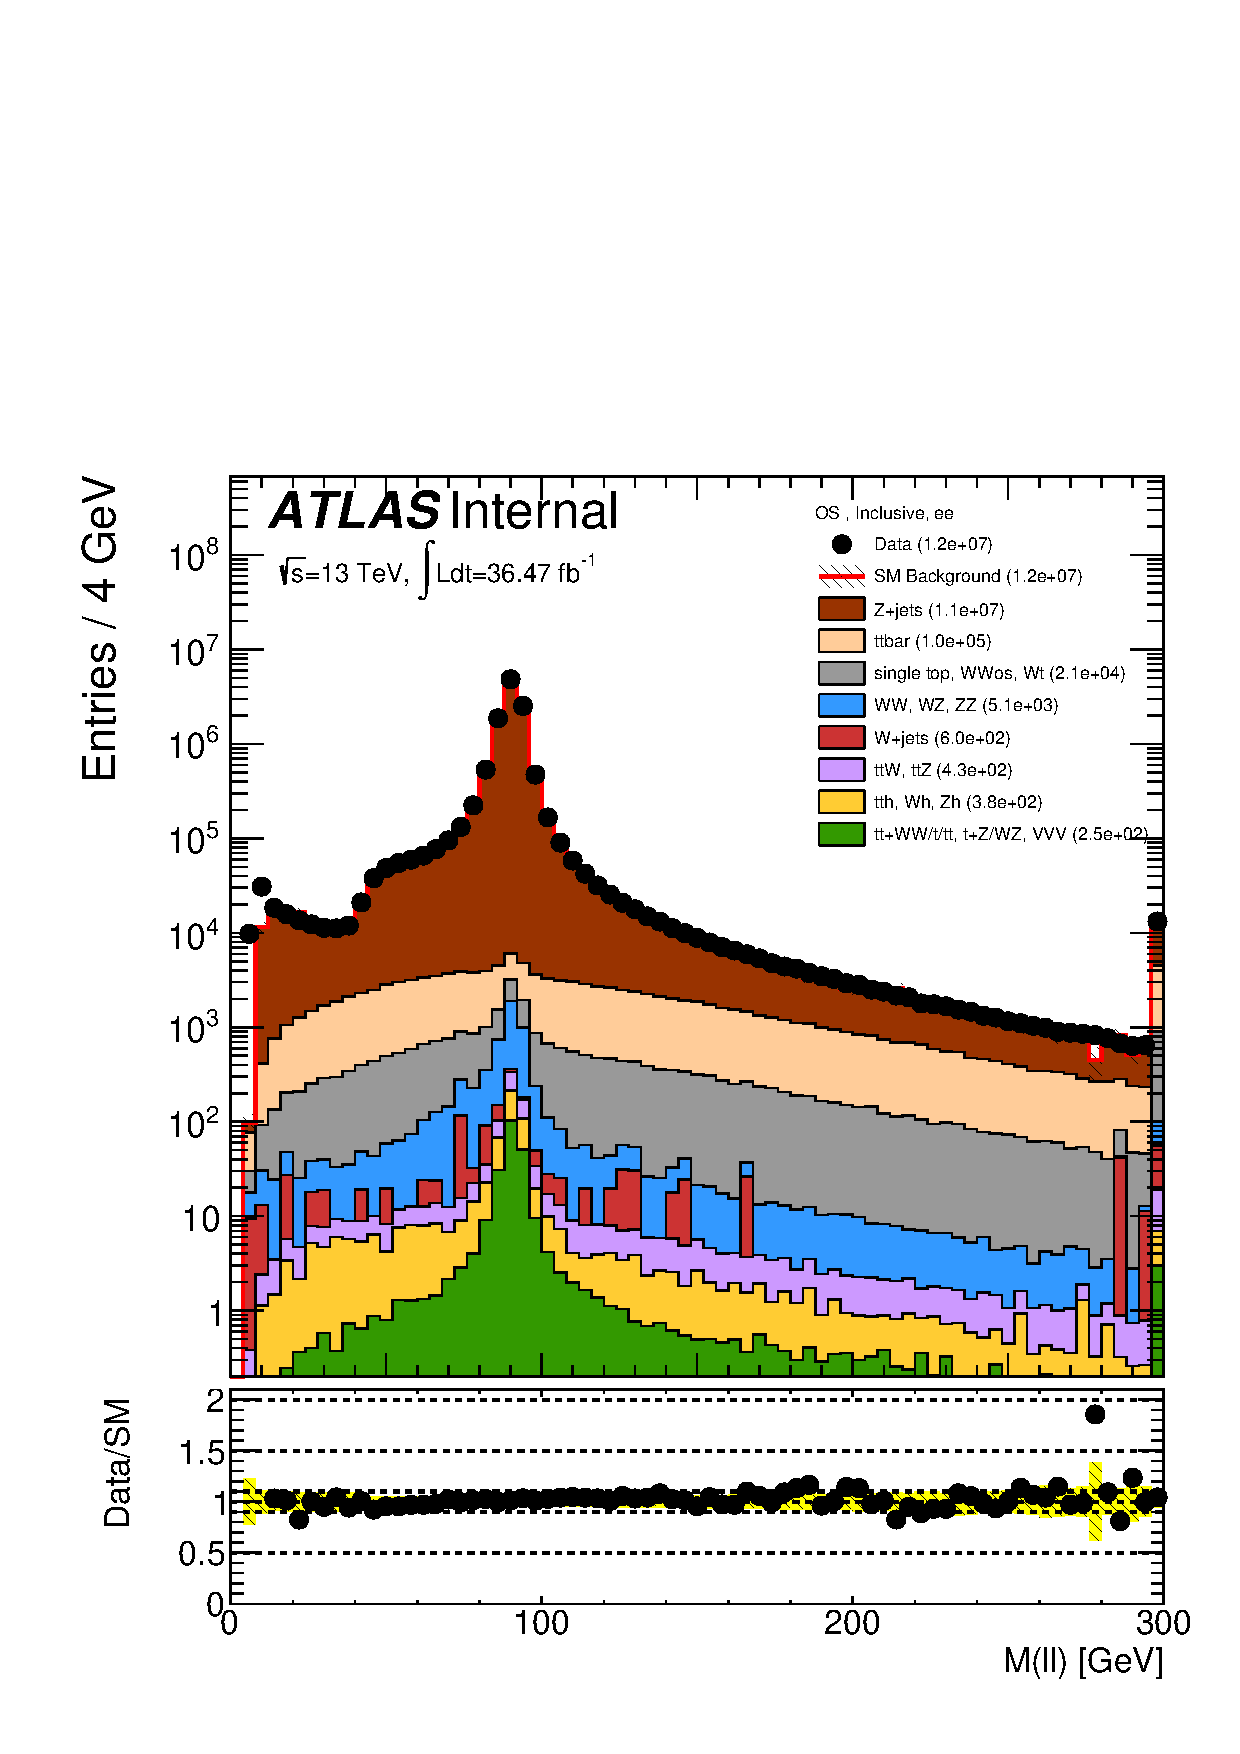
\includegraphics[width=0.4\textwidth]{DATAMC/Mll_ee_Incl_OS_log.pdf}}
{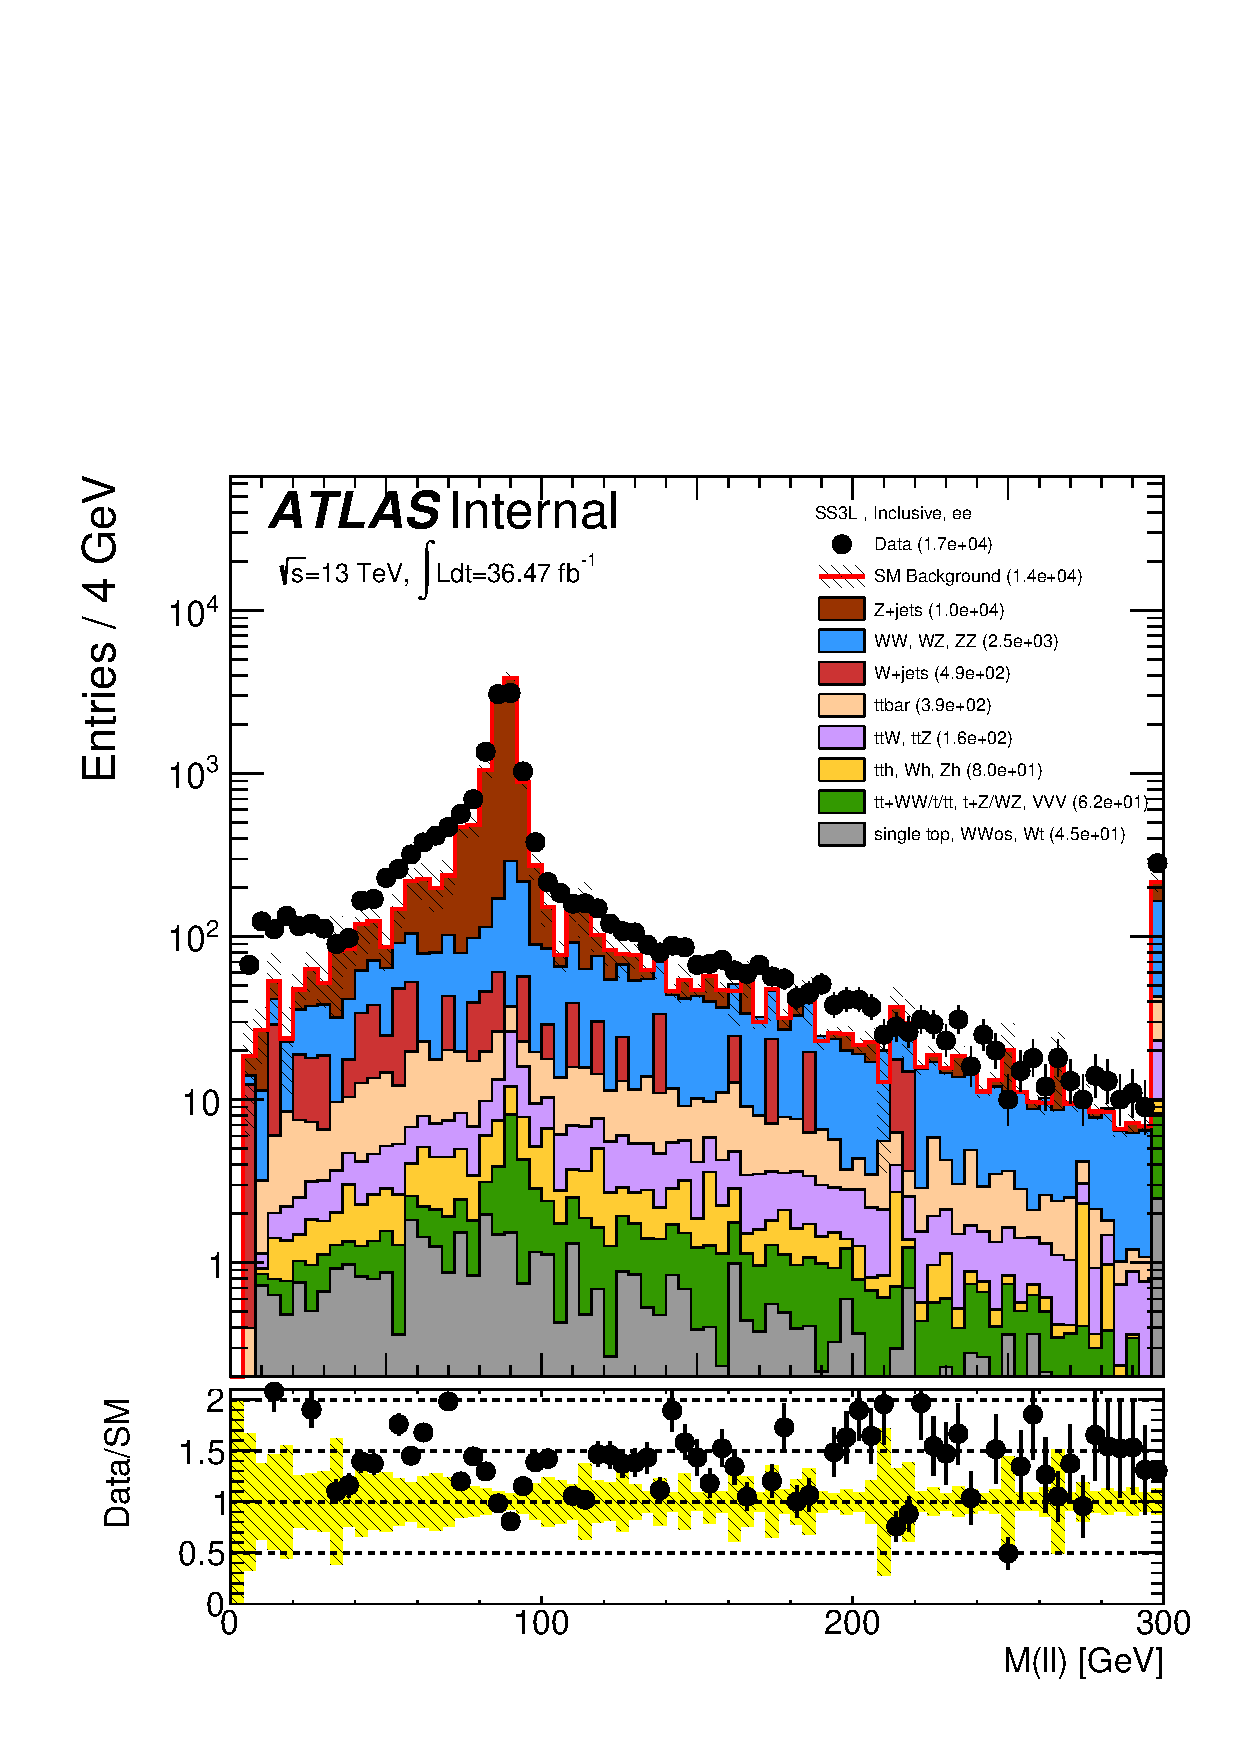
\includegraphics[width=0.4\textwidth]{DATAMC/Mll_ee_Incl_SS3L_log.pdf}}
{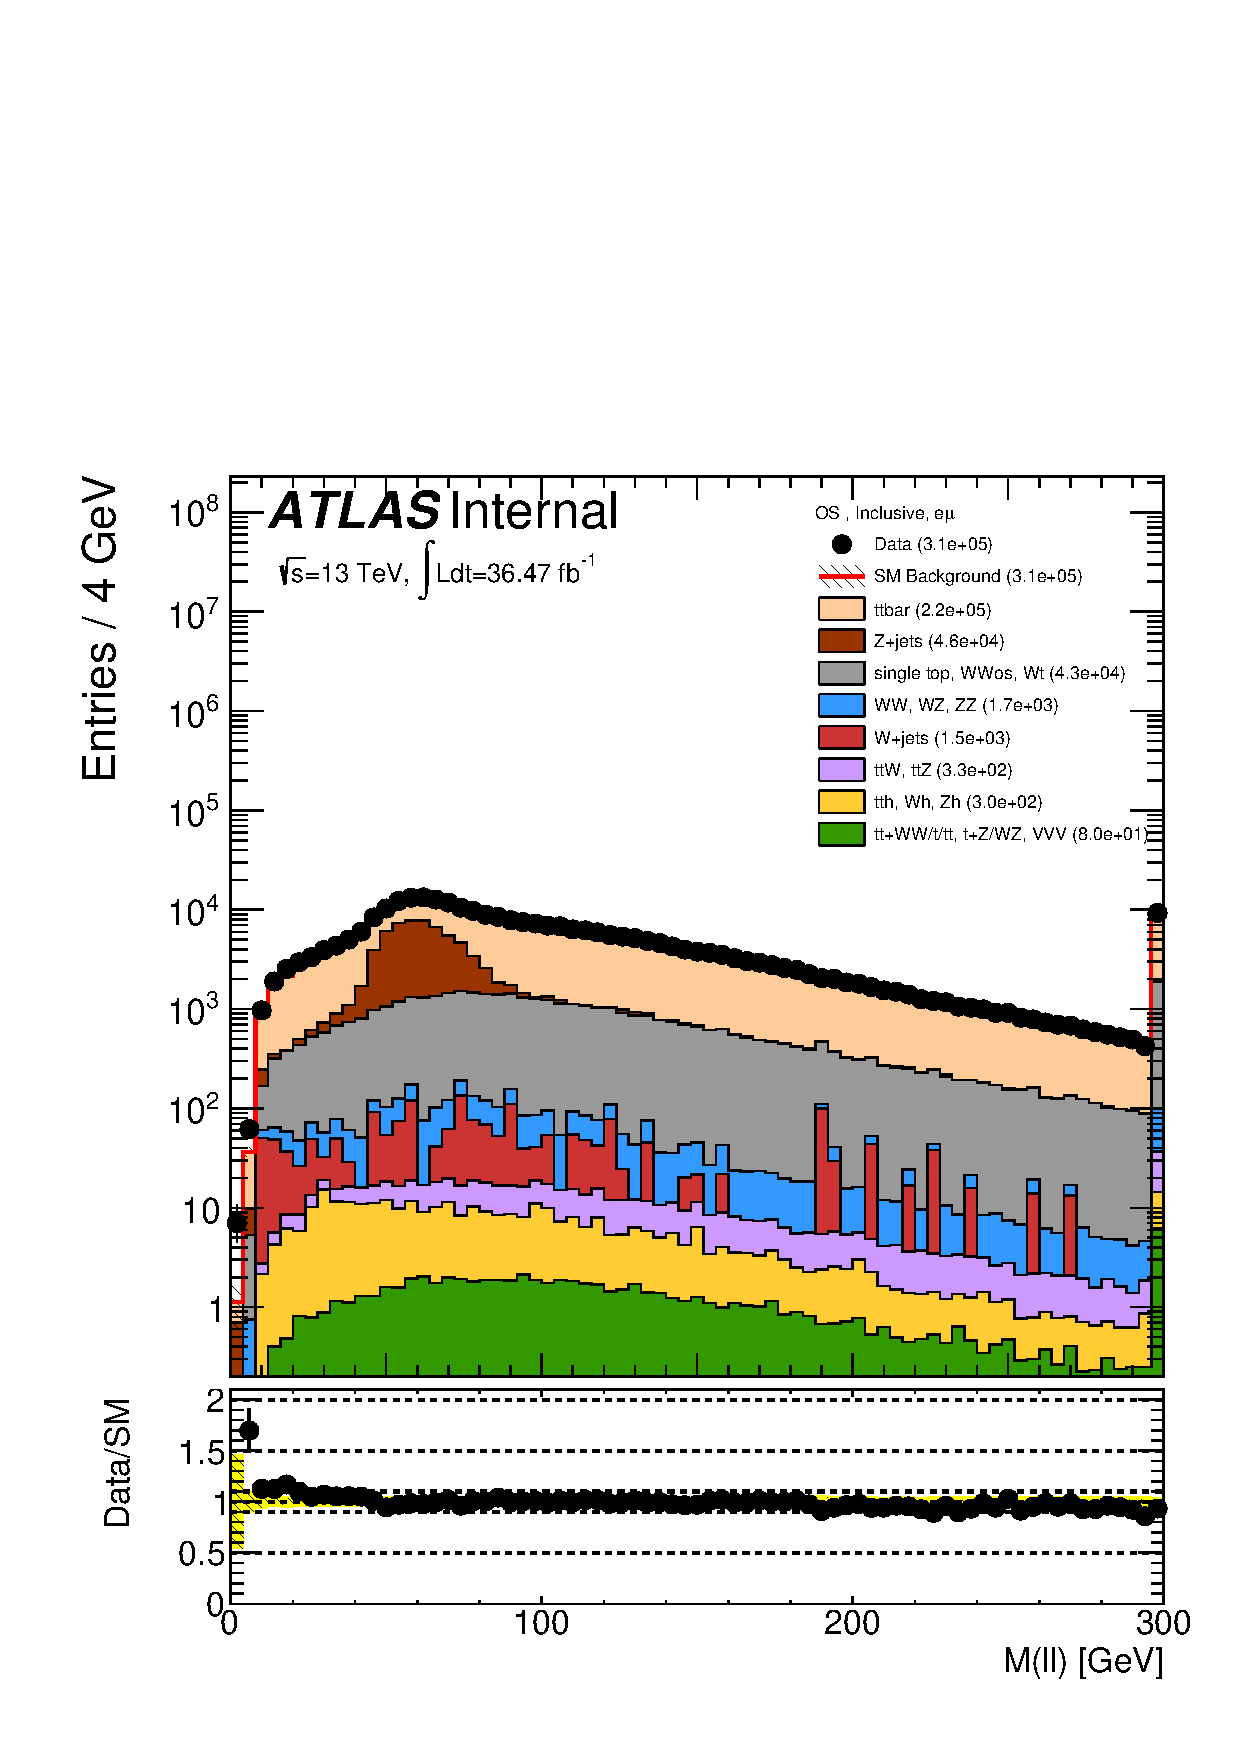
\includegraphics[width=0.4\textwidth]{DATAMC/Mll_em_Incl_OS_log.pdf}}
{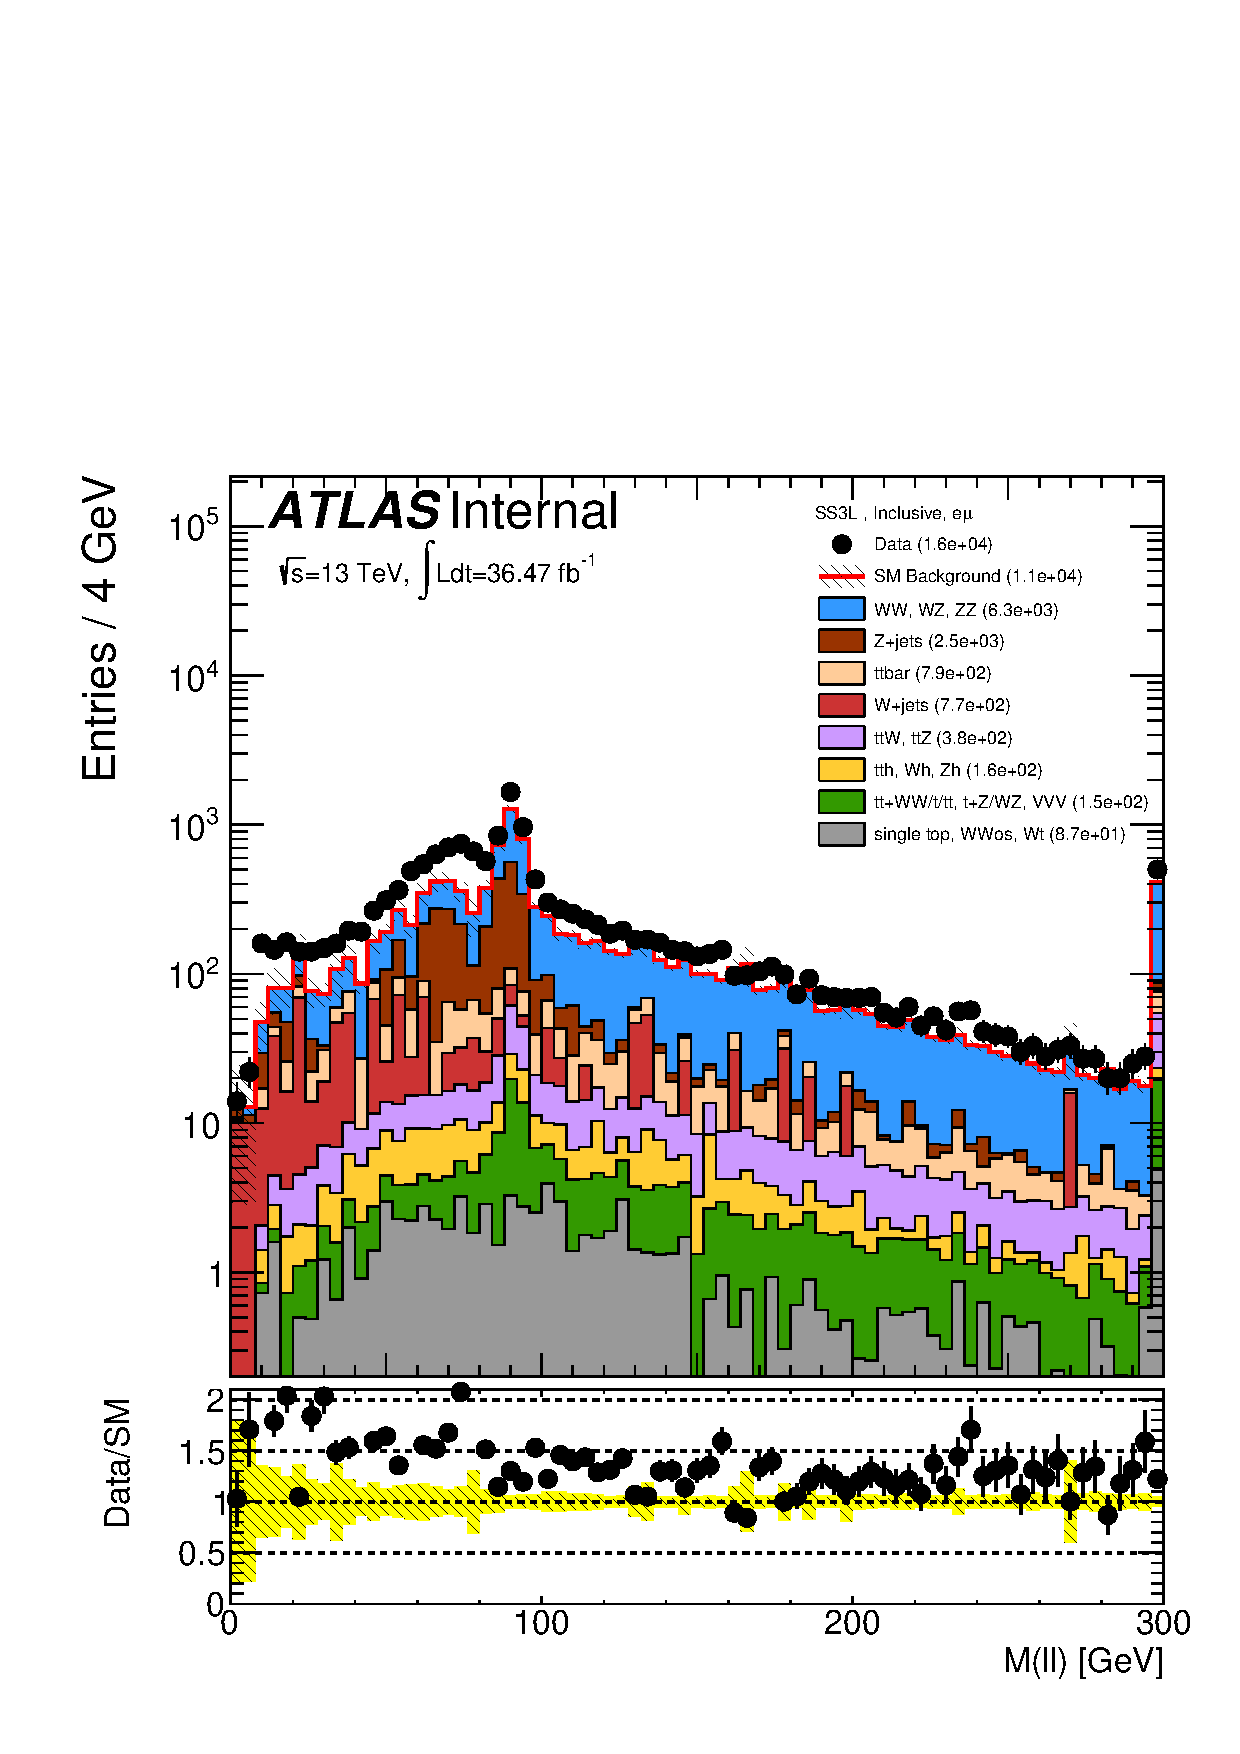
\includegraphics[width=0.4\textwidth]{DATAMC/Mll_em_Incl_SS3L_log.pdf}}
{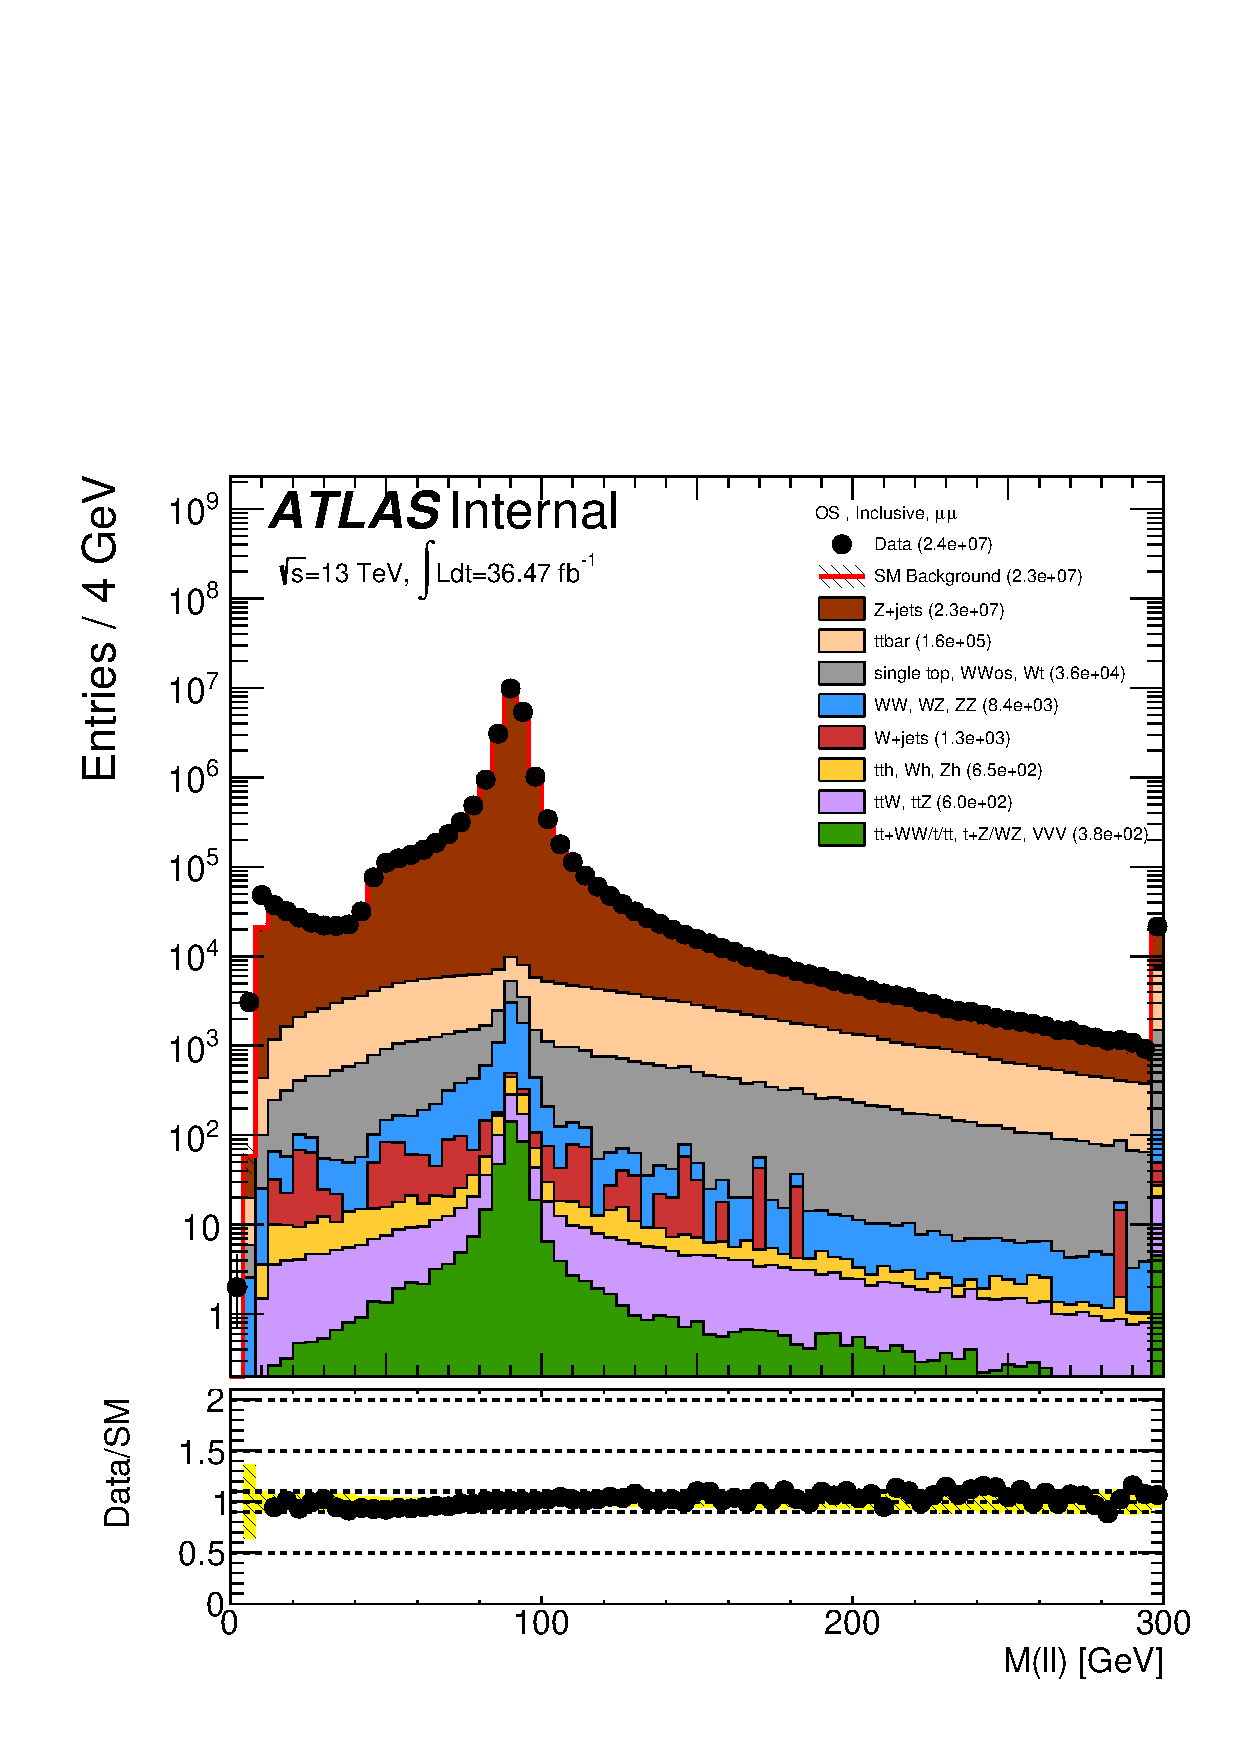
\includegraphics[width=0.4\textwidth]{DATAMC/Mll_mm_Incl_OS_log.pdf}}
{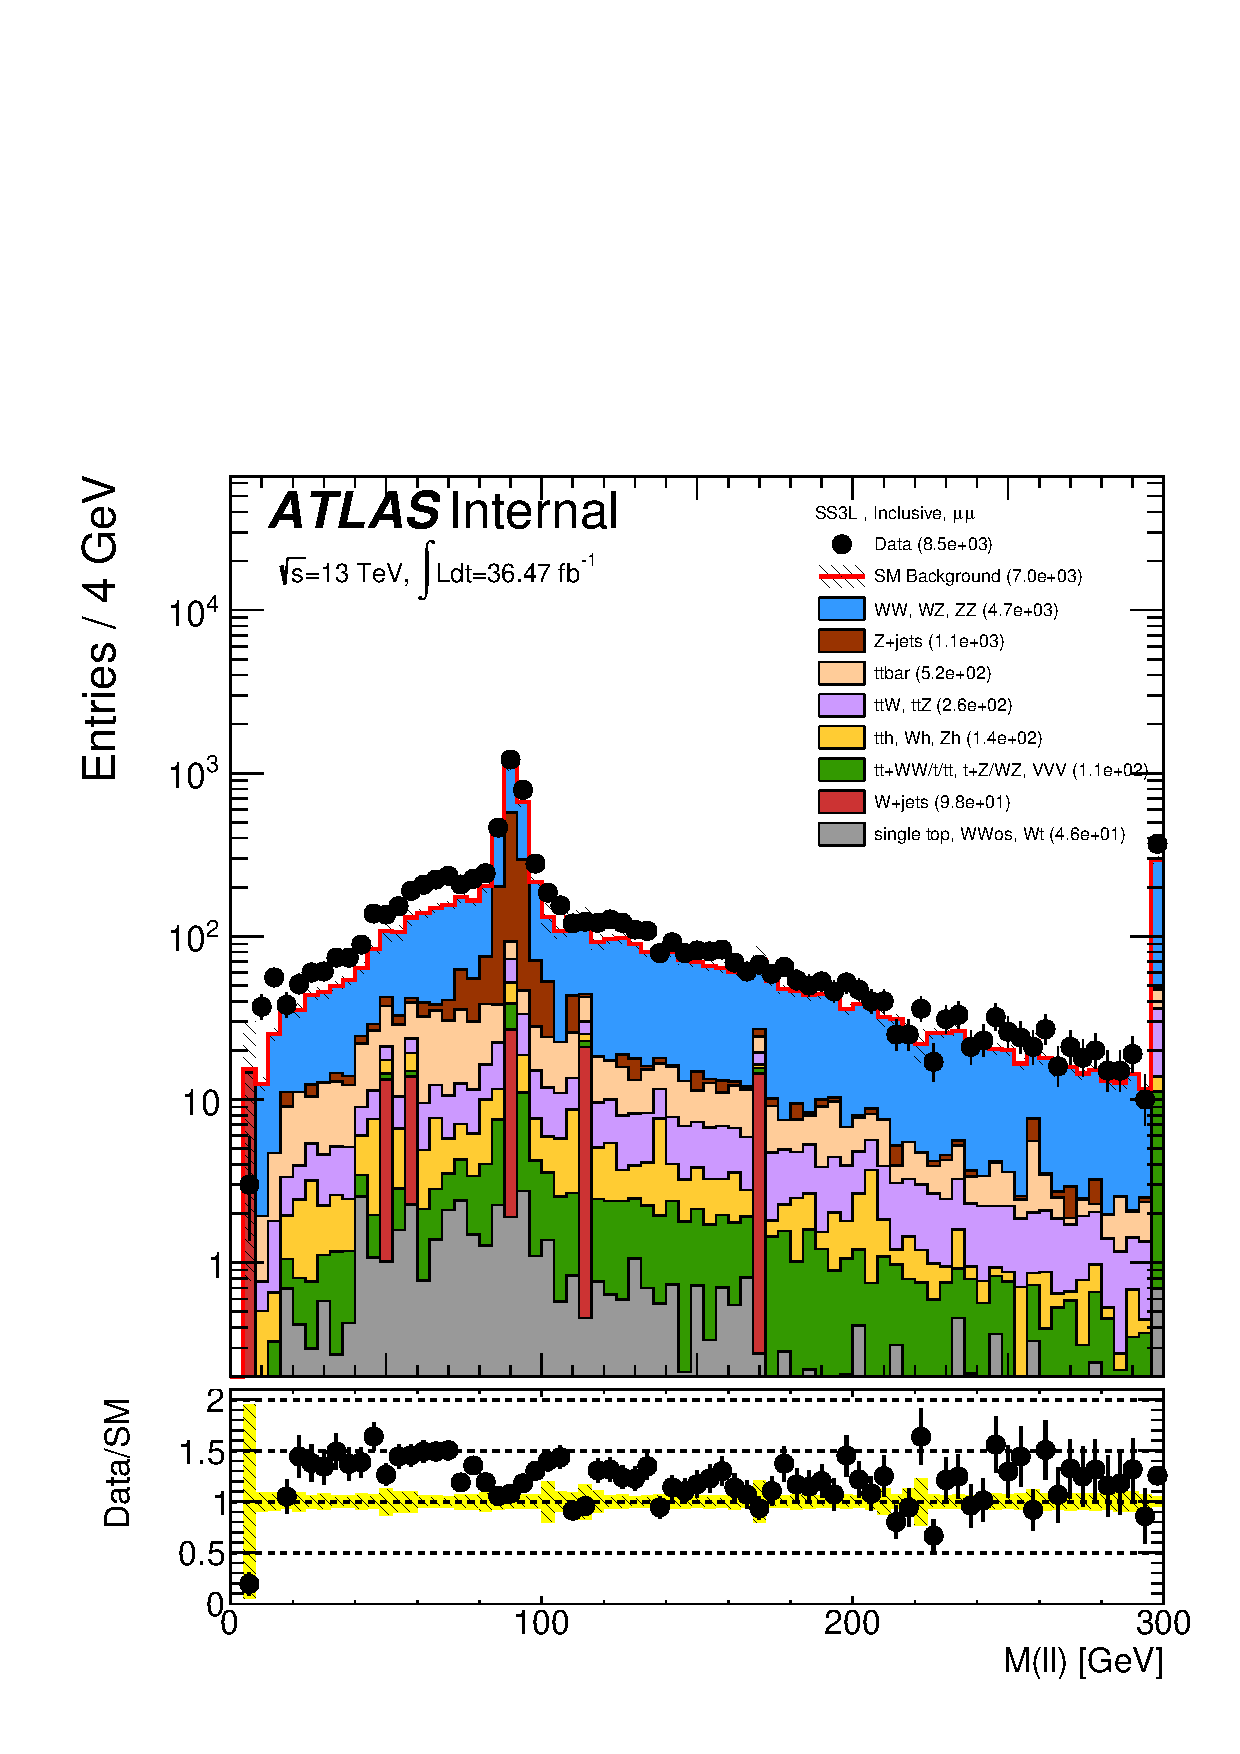
\includegraphics[width=0.4\textwidth]{DATAMC/Mll_mm_Incl_SS3L_log.pdf}}
\caption{Dilepton invariant mass distributions for opposite-sign (left) and same-sign (right) pairs for events selected in the $ee$ (top), $e\mu$ (center) and $\mu\mu$ (bottom) channels. No low-mass Drell-Yan sample is included. 
 The prediction is taken from MC only.
Only luminosity and MC statistical uncertainties are included.
}
\label{fig:dataMC_2lep}
\end{figure}

\begin{figure}[htb!]
\centering
{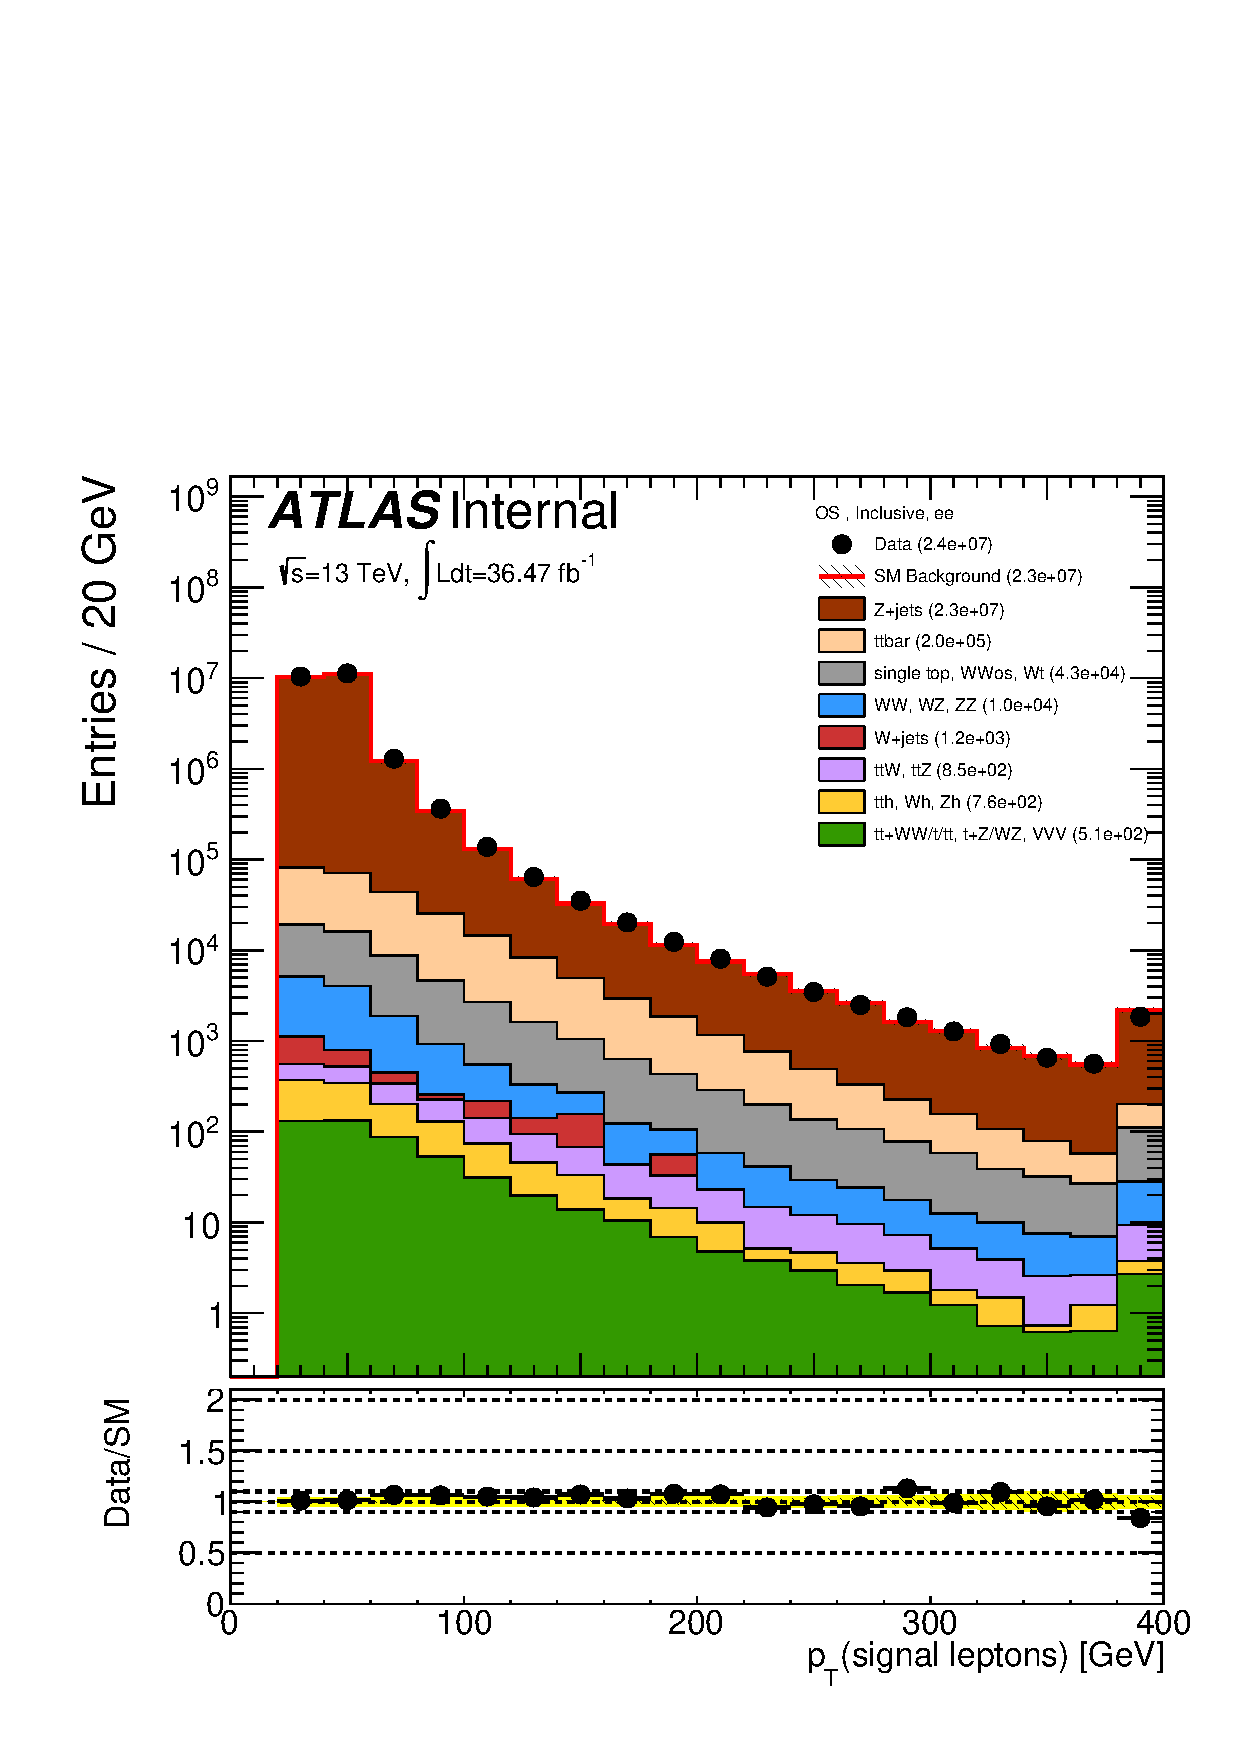
\includegraphics[width=0.4\textwidth]{DATAMC/LEPPt_ee_Incl_OS_log.pdf}}
{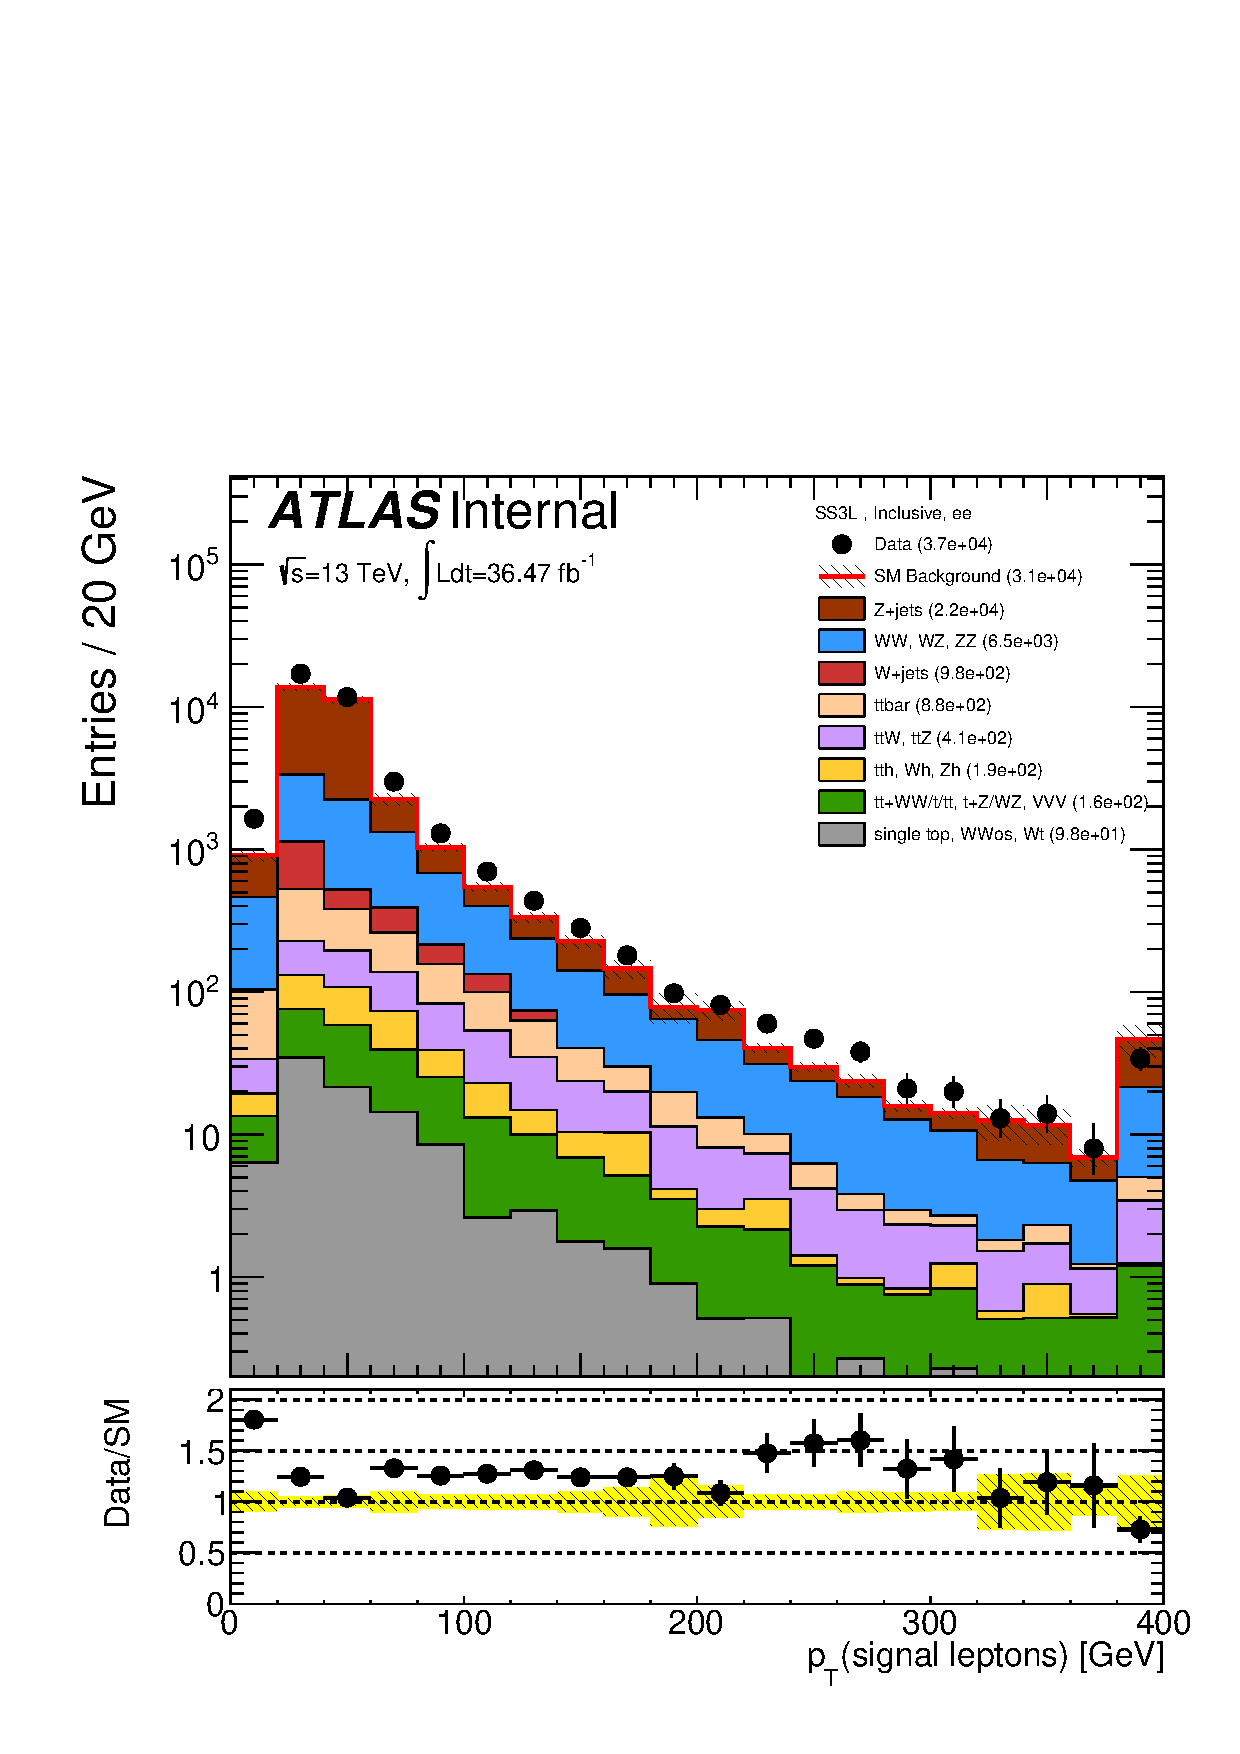
\includegraphics[width=0.4\textwidth]{DATAMC/LEPPt_ee_Incl_SS3L_log.pdf}}
{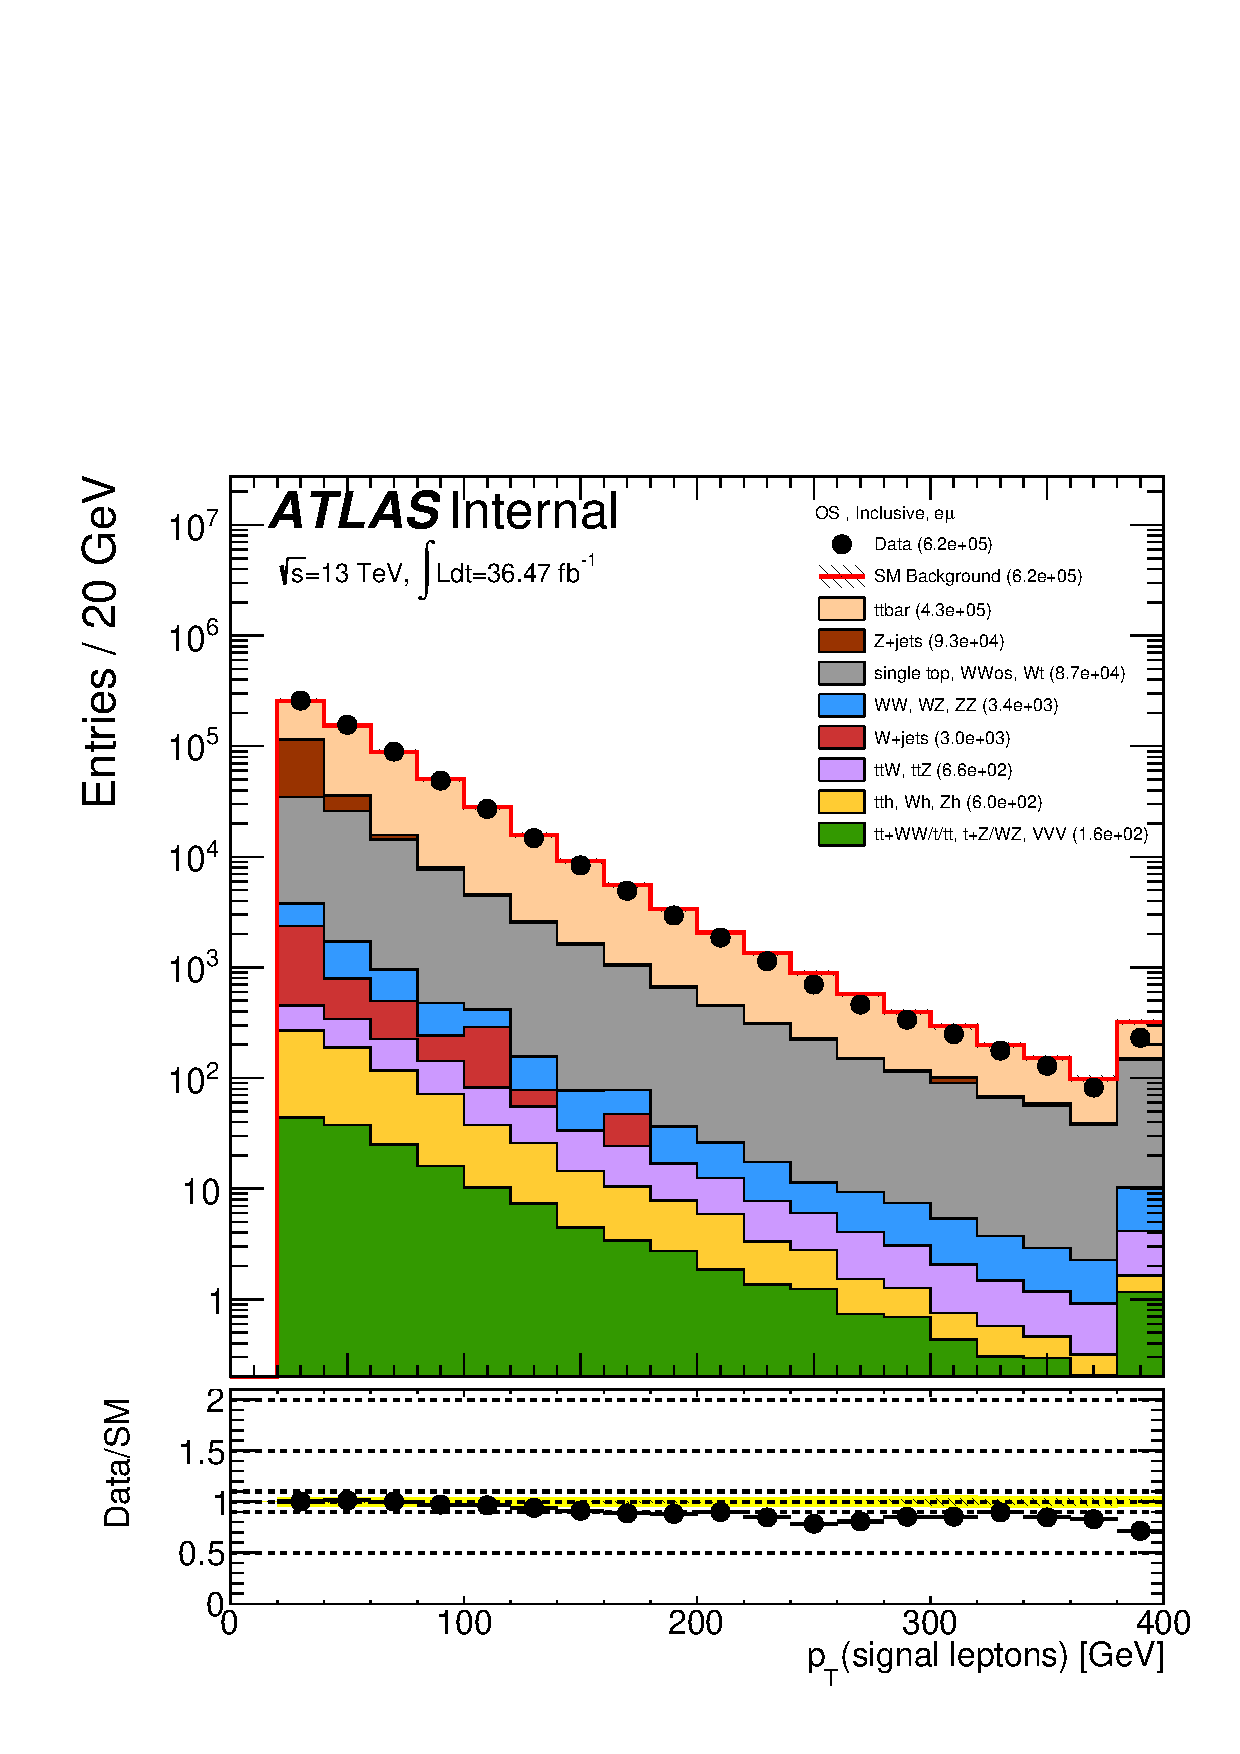
\includegraphics[width=0.4\textwidth]{DATAMC/LEPPt_em_Incl_OS_log.pdf}}
{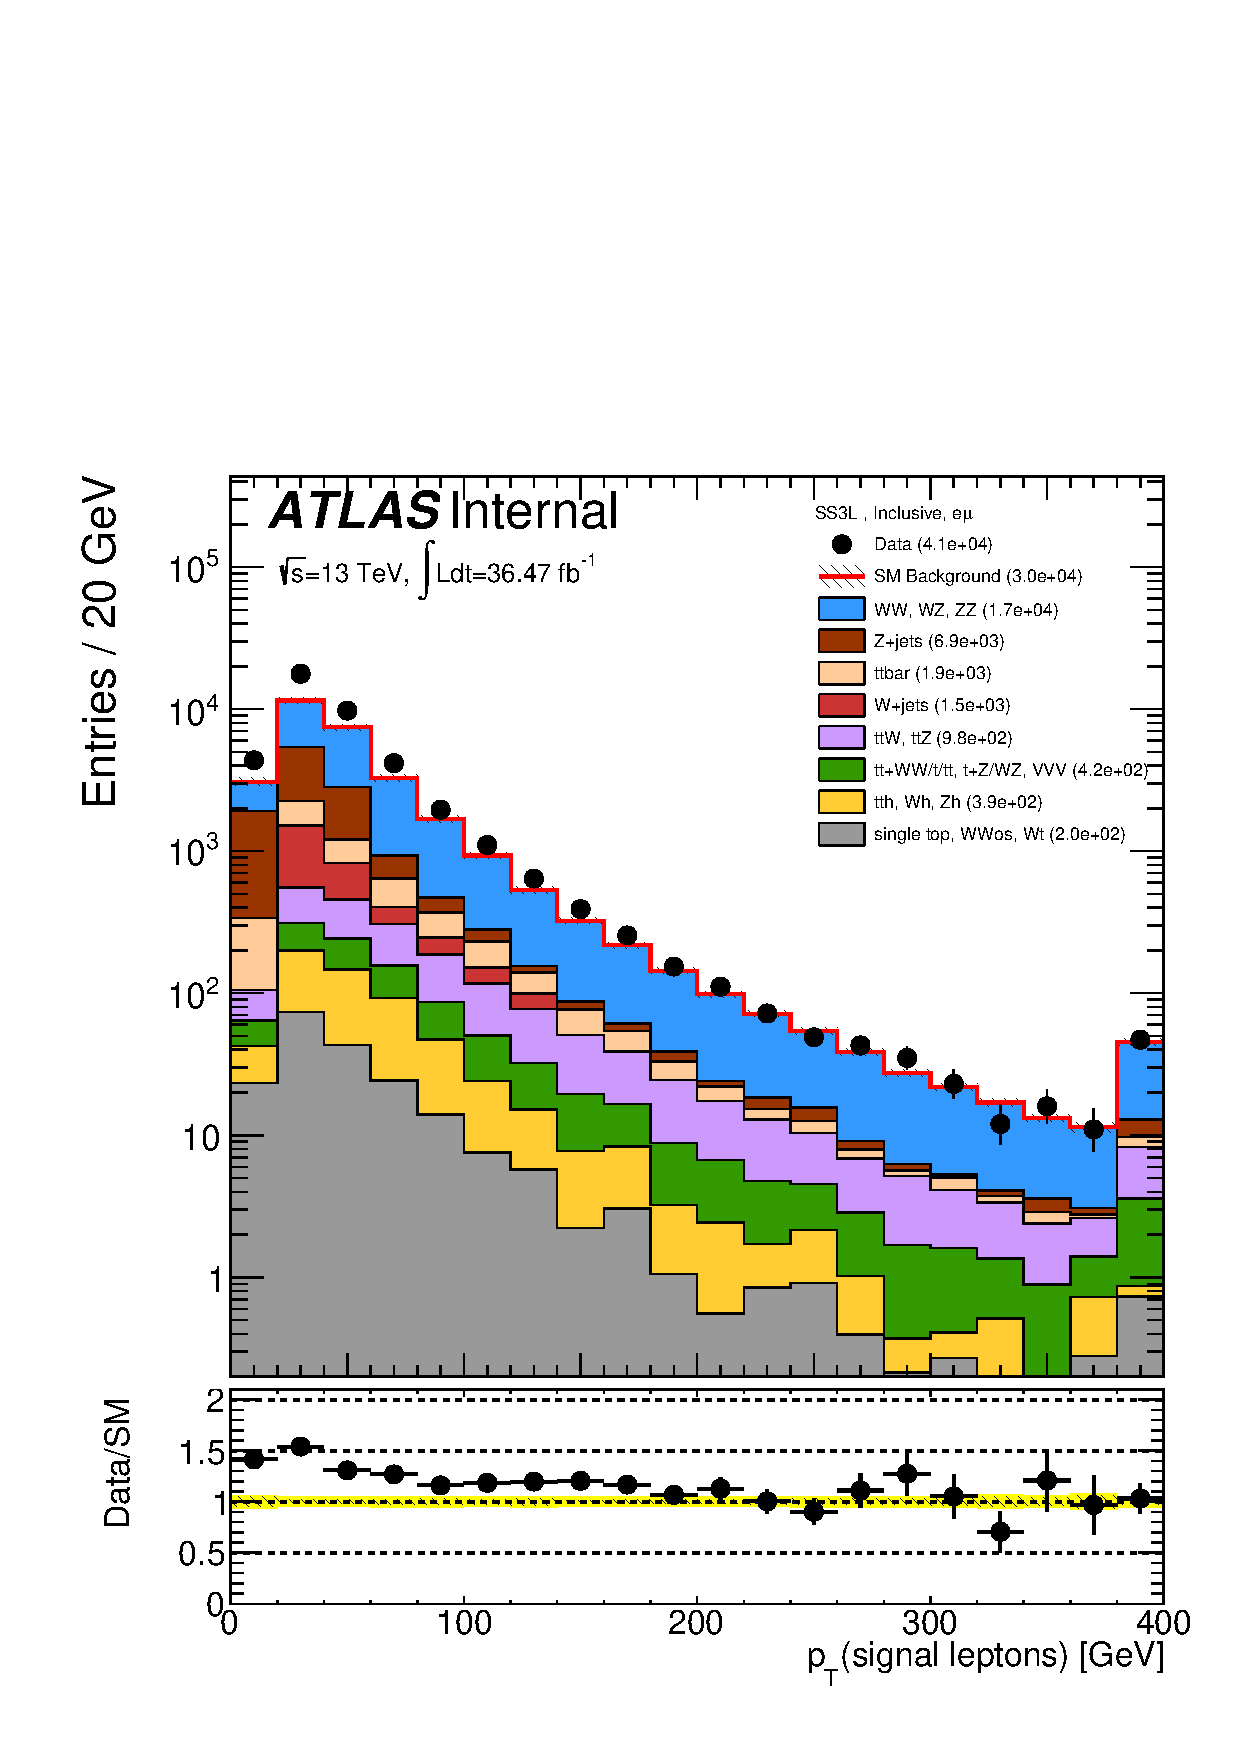
\includegraphics[width=0.4\textwidth]{DATAMC/LEPPt_em_Incl_SS3L_log.pdf}}
{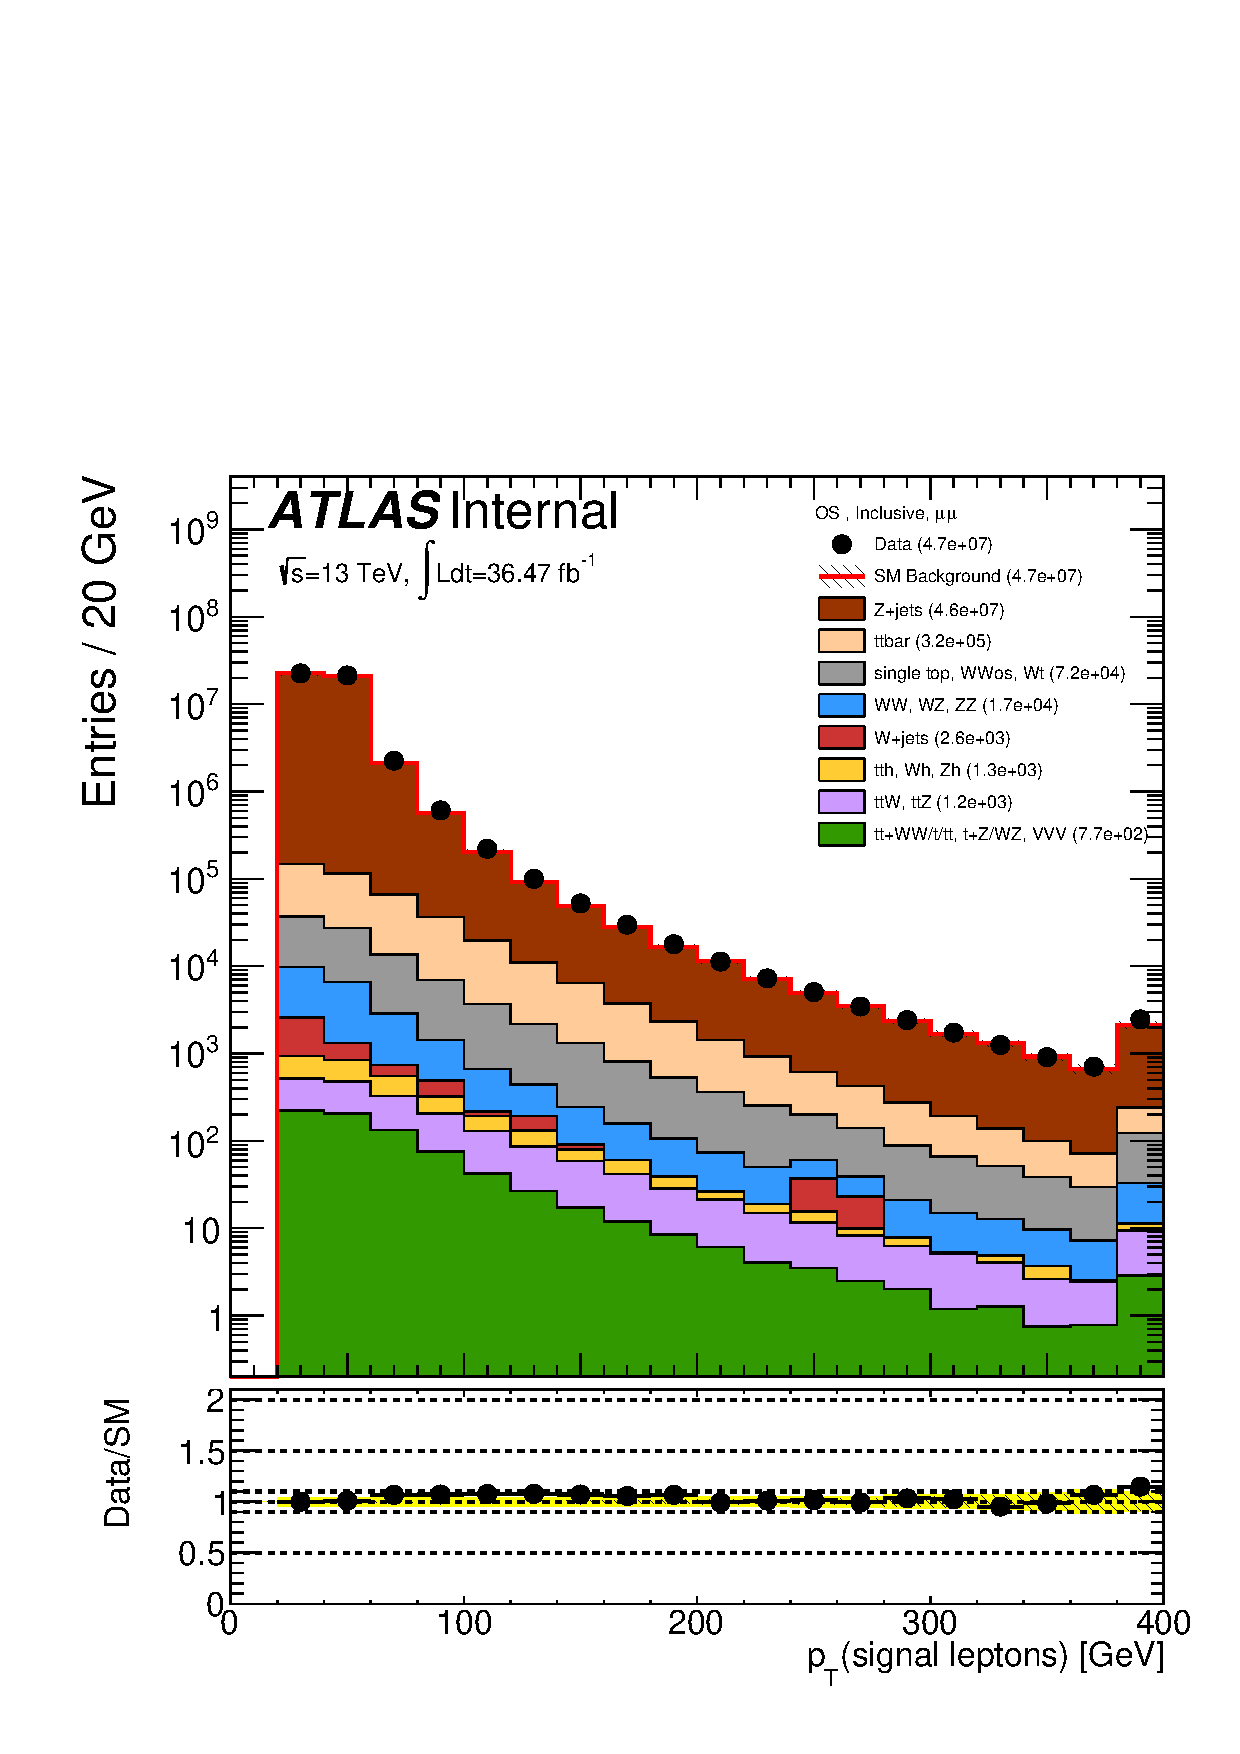
\includegraphics[width=0.4\textwidth]{DATAMC/LEPPt_mm_Incl_OS_log.pdf}}
{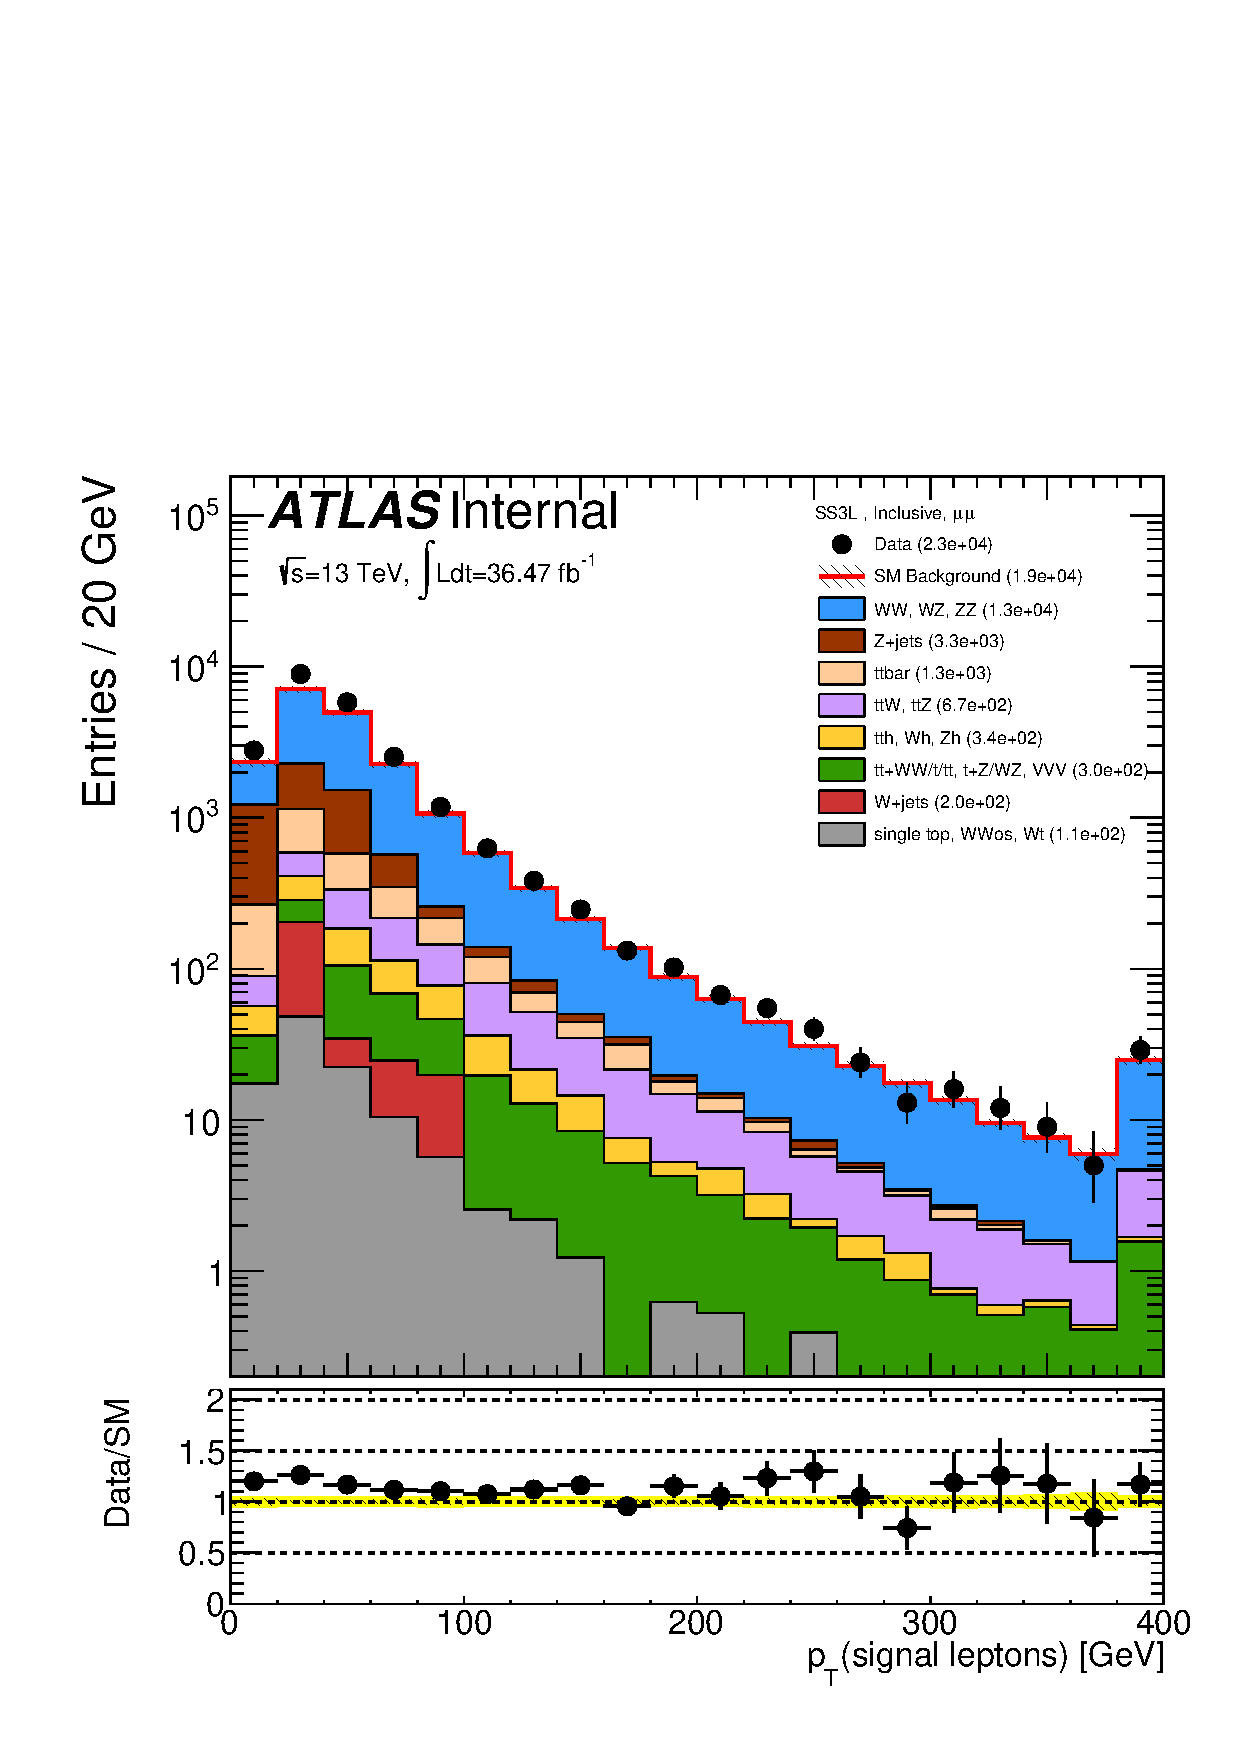
\includegraphics[width=0.4\textwidth]{DATAMC/LEPPt_mm_Incl_SS3L_log.pdf}}
\caption{Signal lepton transverse momentum distributions for opposite-sign (left) and same-sign (right) pairs for events selected in the $ee$ (top), $e\mu$ (center) and $\mu\mu$ (bottom) channels.  The prediction is taken from MC only.
Only luminosity and MC statistical uncertainties are included.
}
\label{fig:dataMC_lep1}
\end{figure}

\begin{figure}[htb!]
\centering
{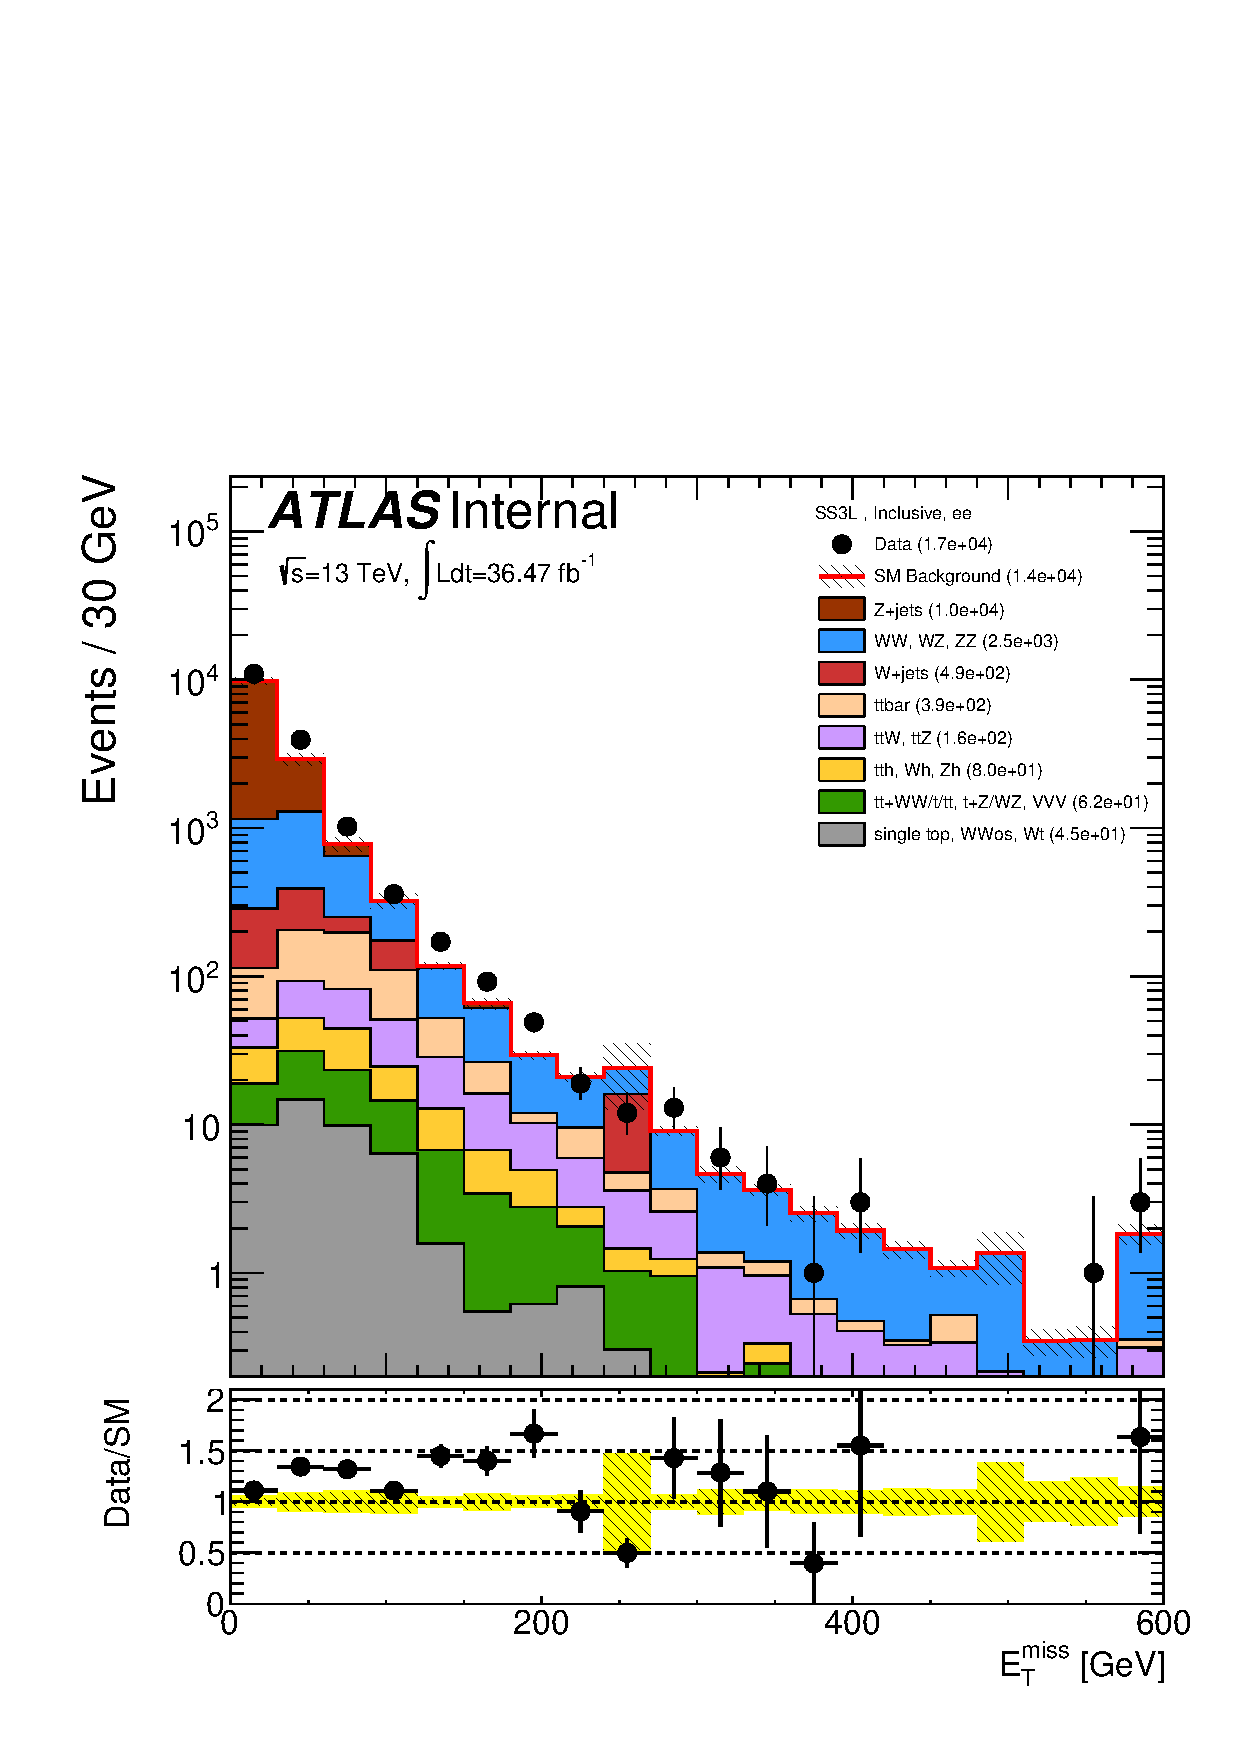
\includegraphics[width=0.4\textwidth]{DATAMC/MET_ee_Incl_SS3L_log.pdf}}
{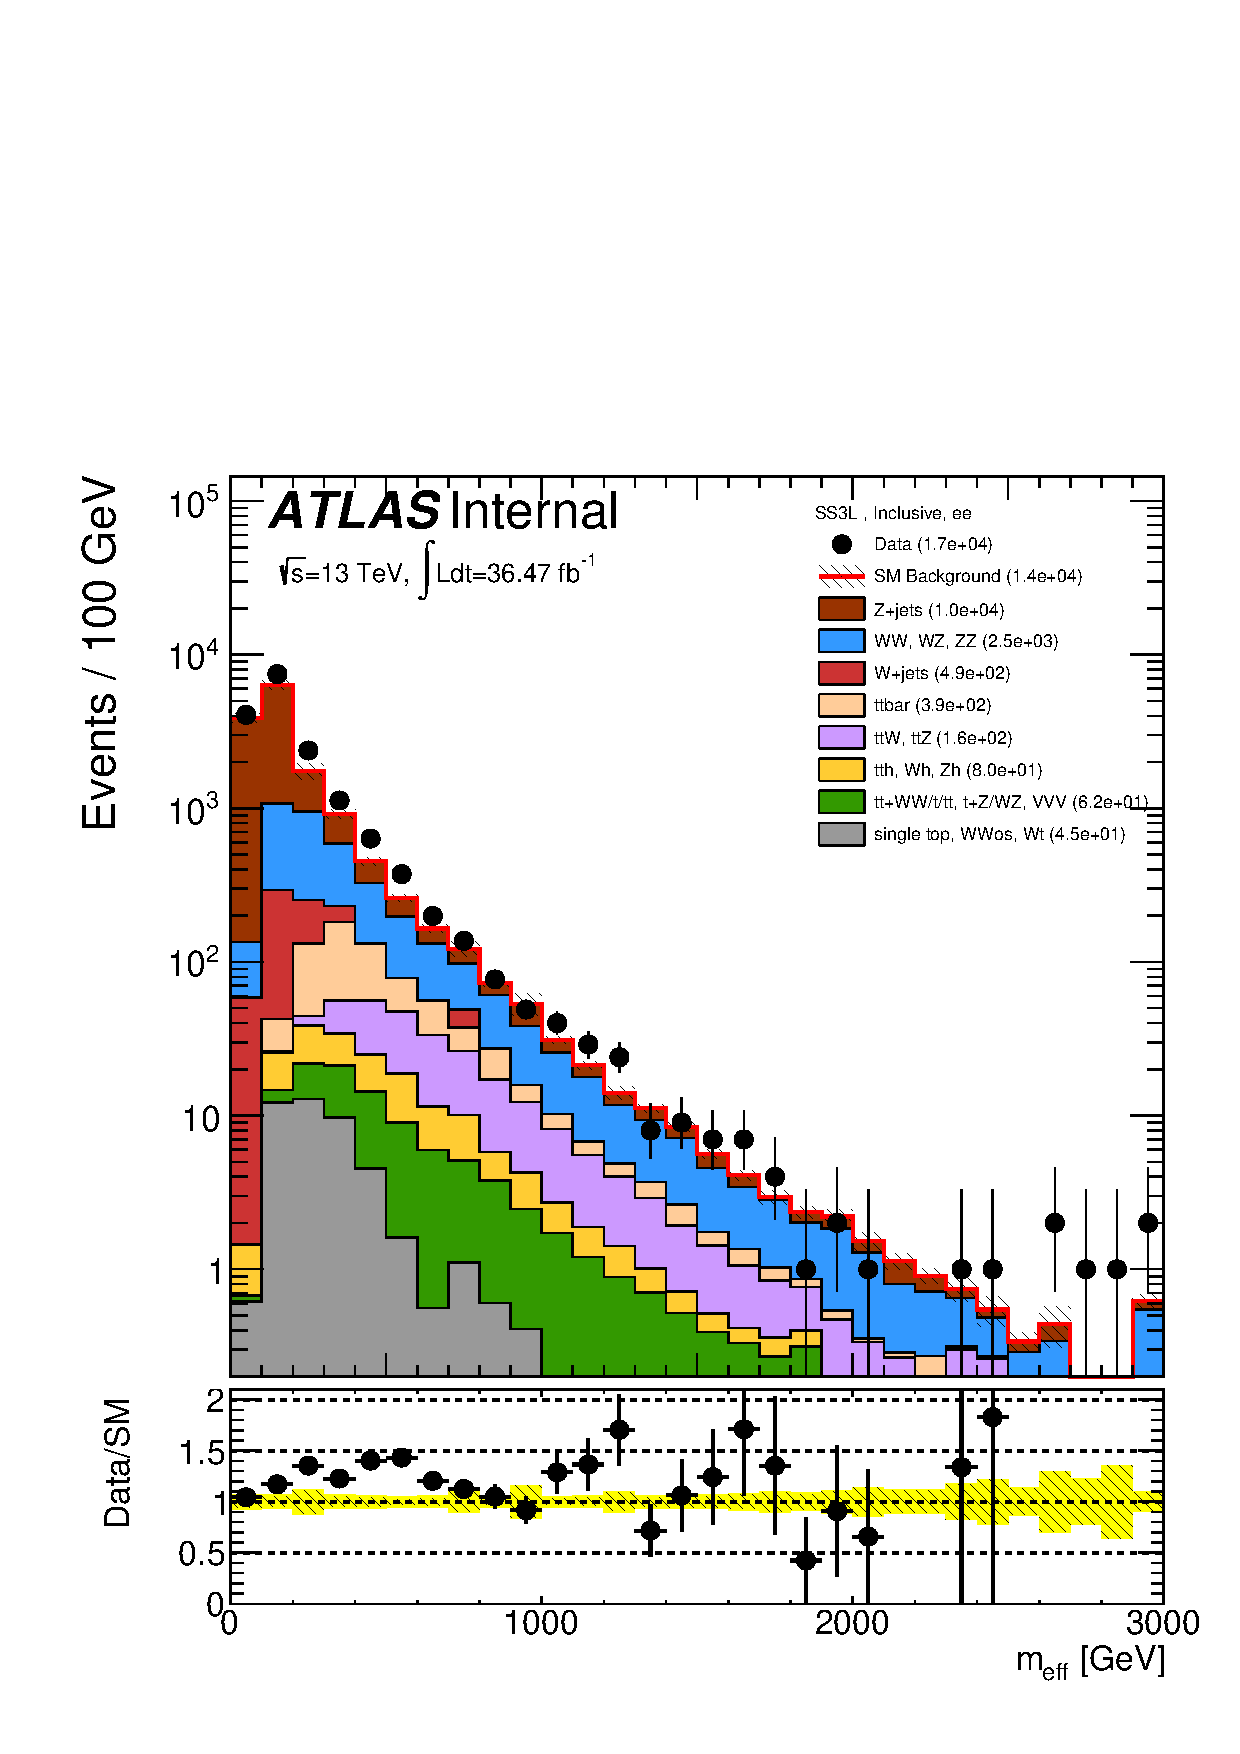
\includegraphics[width=0.4\textwidth]{DATAMC/Meff_ee_Incl_SS3L_log.pdf}}
{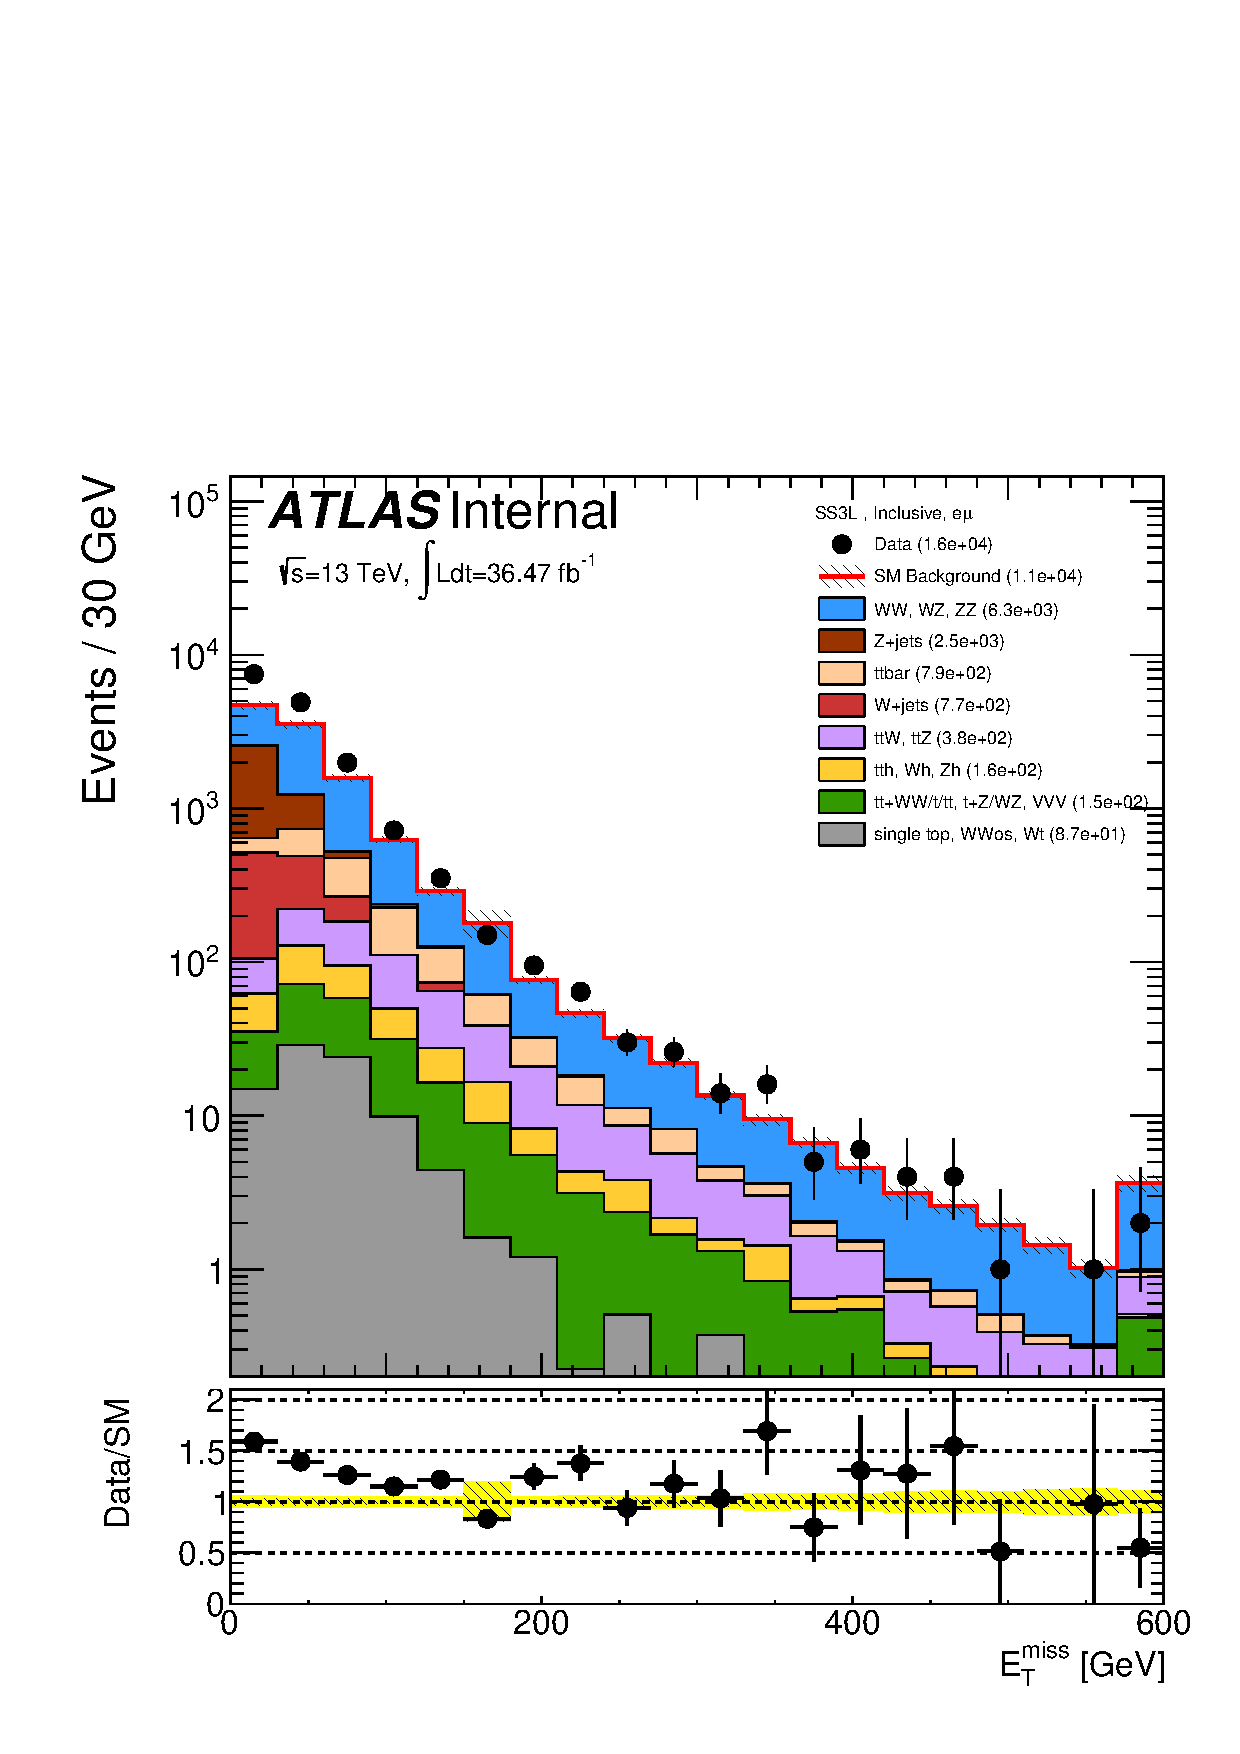
\includegraphics[width=0.4\textwidth]{DATAMC/MET_em_Incl_SS3L_log.pdf}}
{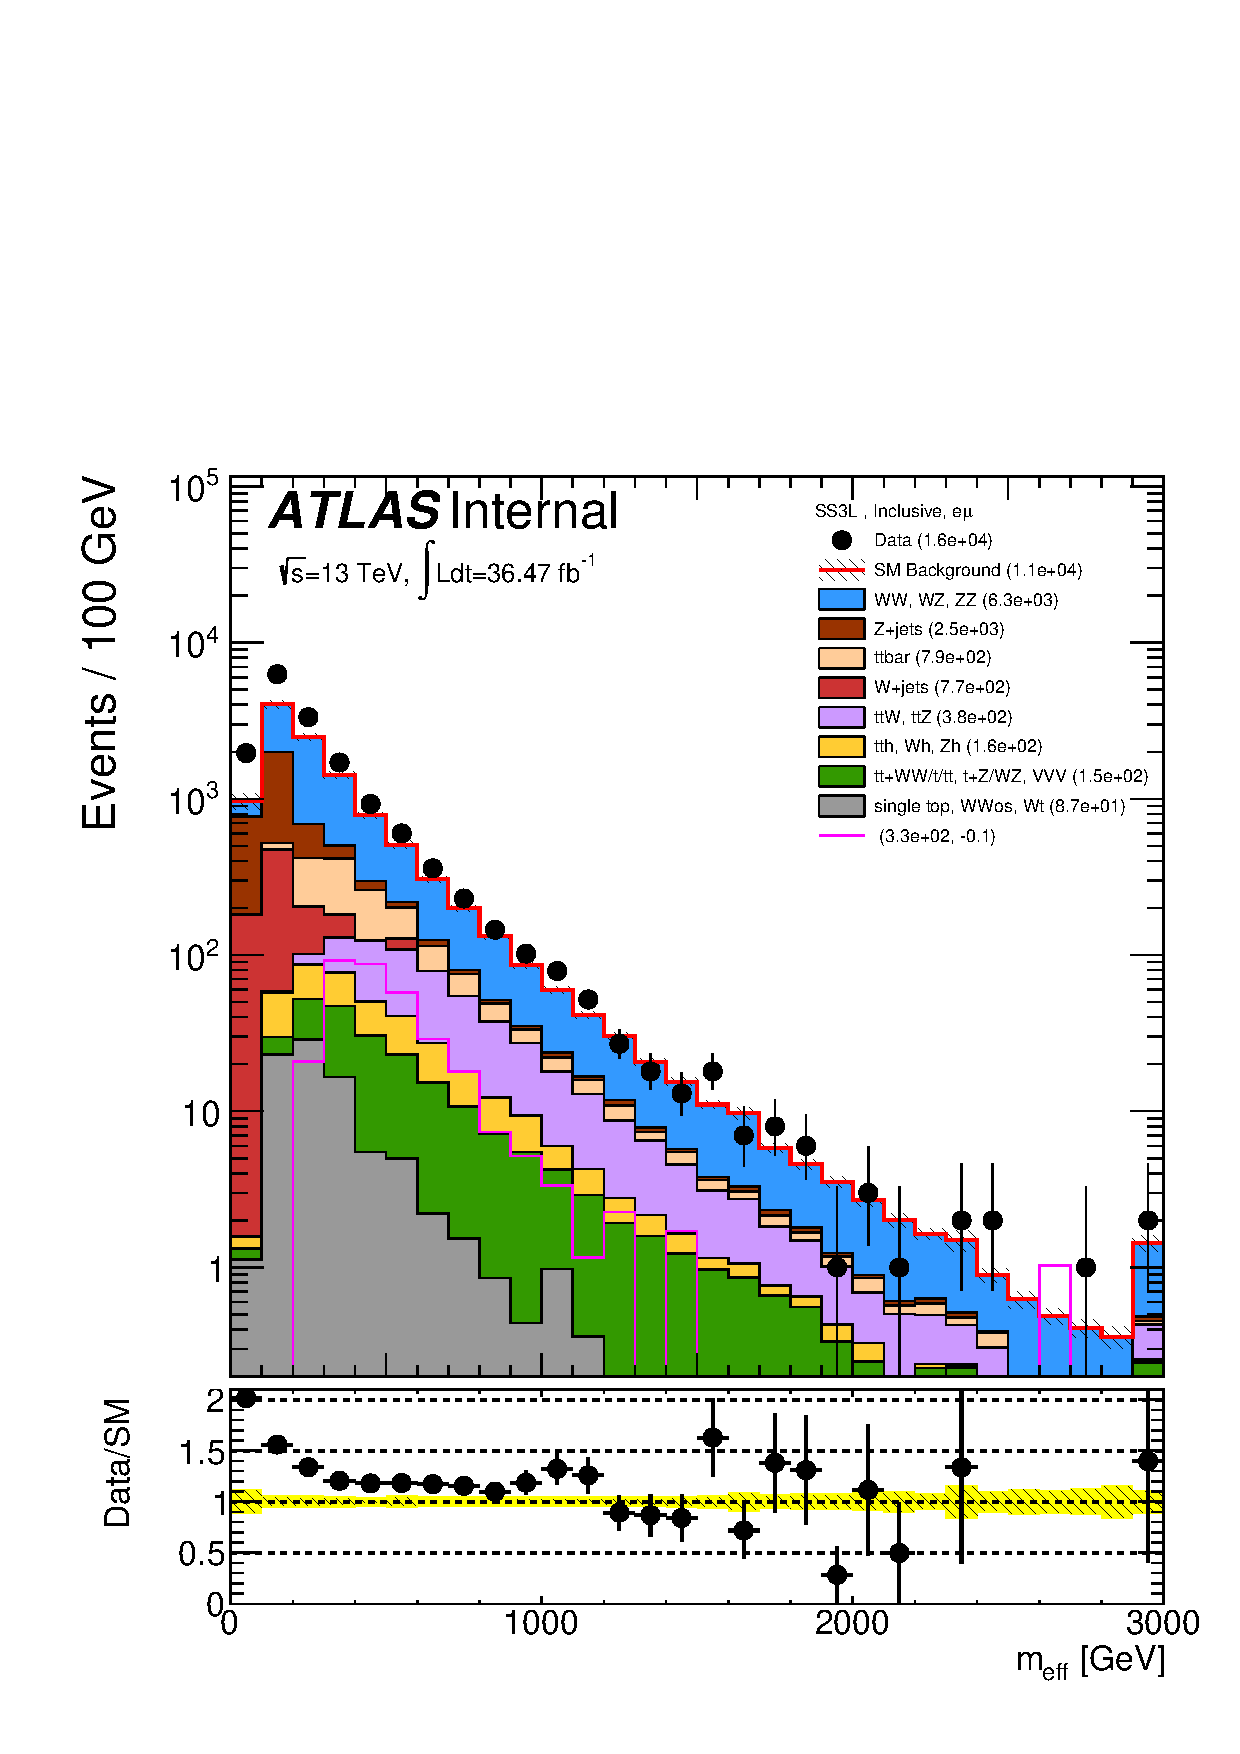
\includegraphics[width=0.4\textwidth]{DATAMC/Meff_em_Incl_SS3L_log.pdf}}
{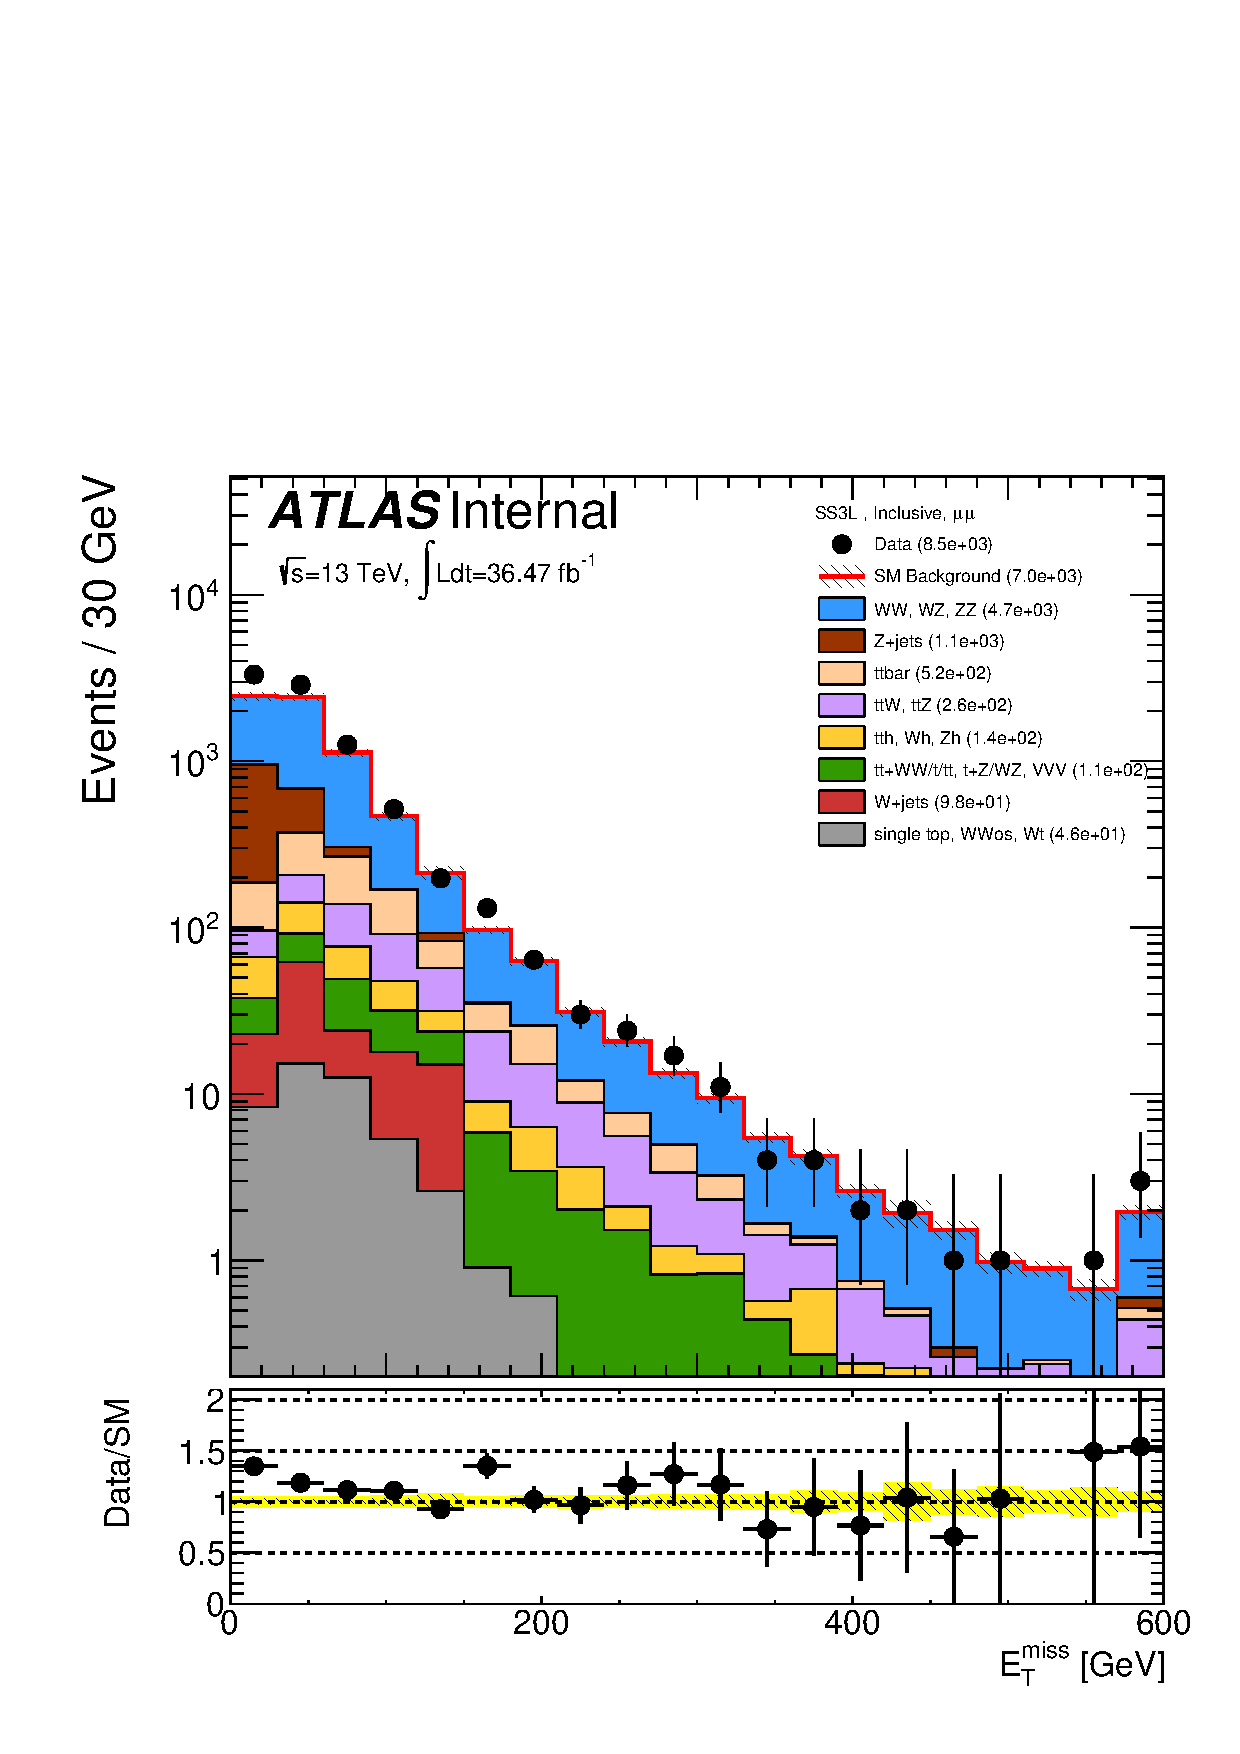
\includegraphics[width=0.4\textwidth]{DATAMC/MET_mm_Incl_SS3L_log.pdf}}
{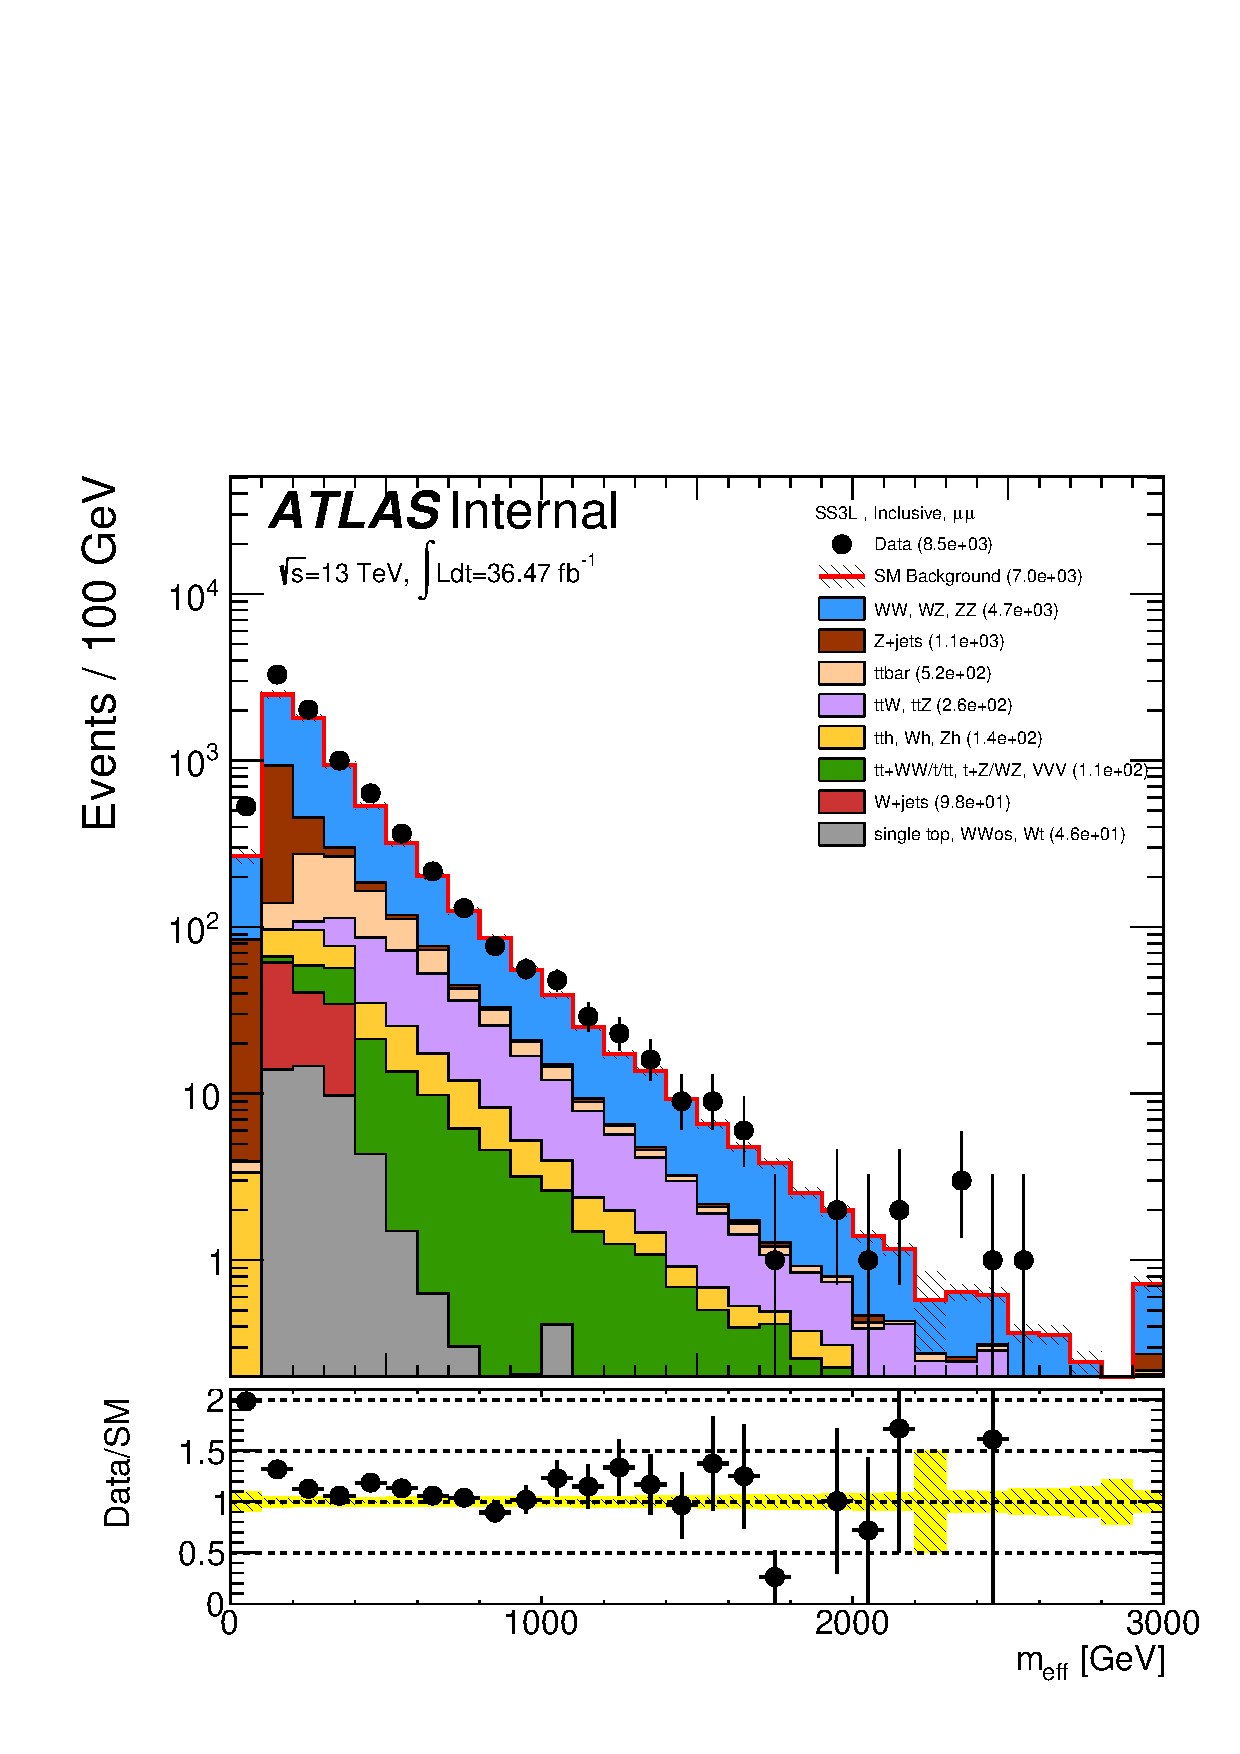
\includegraphics[width=0.4\textwidth]{DATAMC/Meff_mm_Incl_SS3L_log.pdf}}
\caption{Distributions of the $\met$ (left) and effective mass (right) for events selected in the $ee$ (top), $e\mu$ (center) and $\mu\mu$ (bottom) channels. 
 The prediction is taken from MC only.
 Only luminosity and MC statistical uncertainties are included.
}
\label{fig:dataMC_metmeff}
\end{figure}
